%!TEX root = ../Thesis.tex
%% Basierend auf TeXnicCenter-Vorlage von Mark Müller
%%                      Willi Nüßer
%%                      Waldemar Penner     
%%                      Ulrich Reus
%%                      Frank Plass
%%                      Oliver Tribeß 
%%                      Daniel Hintze     
%%%%%%%%%%%%%%%%%%%%%%%%%%%%%%%%%%%%%%%%%%%%%%%%%%%%%%%%%%%%%%%%%%%%%%%

% Wählen Sie die Optionen aus, indem Sie % vor der Option entfernen  
% Dokumentation des KOMA-Script-Packets: scrguide

%%%%%%%%%%%%%%%%%%%%%%%%%%%%%%%%%%%%%%%%%%%%%%%%%%%%%%%%%%%%%%%%%%%%%%%
%% Optionen zum Layout des Artikels                                  %%
%%%%%%%%%%%%%%%%%%%%%%%%%%%%%%%%%%%%%%%%%%%%%%%%%%%%%%%%%%%%%%%%%%%%%%%
\documentclass[%
    paper=A4,         % alle weiteren Papierformat einstellbar
    fontsize=11pt,    % Schriftgröße (12pt, 11pt (Standard))
    BCOR12mm,         % Bindekorrektur, bspw. 1 cm
    DIV14,            % breiter Satzspiegel
    parskip=half*,    % Absatzformatierung s. scrguide 3.1
    headsepline,      % Trennline zum Seitenkopf
%footsepline,     % Trennline zum Seitenfuß
%normalheadings,  % Überschriften etwas kleiner (smallheadings)
    listof=totoc,     % Tabellen & Abbildungsverzeichnis ins Inhaltsverzeichnis
%bibtotoc,        % Literaturverzeichnis im Inhalt 
%draft            % Überlangen Zeilen in Ausgabe gekennzeichnet
    footinclude=false,% Fußzeile in die Satzspiegelberechnung einbeziehen
    headinclude=true, % Kopfzeile in die Satzspiegelberechnung einbeziehen
    final             % draft beschleunigt die Kompilierung
]
{scrartcl}

%\setuptoc{toc}{totoc} % Inhaltsverzeichnis ins Inhaltsverzeichnis

% Neue Deutsche Rechtschreibung und Deutsche Standardtexte
\usepackage[ngerman]{babel}

% Umlaute können verwendet werden
\usepackage[utf8]{inputenc}

% Echte Umlaute
\usepackage[T1]{fontenc}

\usepackage{pifont}% http://ctan.org/pkg/pifont

% Latin Modern Font, Type1-Schriftart für nicht-englische Texte
\usepackage{lmodern}

% 1/2-zeiliger Zeilenabstand
\usepackage[onehalfspacing]{setspace}

% Für die Defenition eigener Kopf- und Fußzeilen
\usepackage{fancyhdr}

% Für die Verwendung von Grafiken
\usepackage[pdftex]{graphicx}

% Bessere Tabellen
\usepackage{tabularx}
\usepackage{longtable}

% Für die Befehle \toprule, \midrule und \bottomrule, z.B. in Tabellen 
\usepackage{booktabs}

% Erlaubt die Benutzung von Farben
\usepackage{color}

% Verbessertes URL-Handling mit \url{http://...}
\usepackage{url}

% Listen ohne Abstände \begin{compactlist}...\end{compactlist}
\usepackage{paralist}

% Ausgabe der aktuellen Uhrzeit für die Draft-Versionen
\usepackage{datetime}

% Deutsche Anführungszeichen
\usepackage[babel,german=quotes]{csquotes}

% Konfiguration der Abbildungs- und Tabellenbezeichnungen
\usepackage[format=hang, font={footnotesize, sf}, labelfont=bf, justification=raggedright,singlelinecheck=false]{caption}

% Verbessert die Lesbarkeit durch Mikrotypografie
\usepackage[activate={true,nocompatibility},final,tracking=true,kerning=true,spacing=true,factor=1100,stretch=10,shrink=10]{microtype}

% Zitate und Quellenverzeichnis
\usepackage[
    bibstyle=authoryear,
    citestyle=authoryear-fhdw,
    firstinits=false,         % false = Vornamen werden ausgeschrieben
    natbib=true,
    urldate=long,             % "besucht am" - Datum
    %url=false,
    date=long,
    dashed=false,
    maxcitenames=3,           % max. Anzahl Autorennamen in Zitaten
    maxbibnames=99,           % max. Anzahl Autorennamen im Quellenverzeichnis
    %backend=bibtex           % Ggf. für ältere Distributionen bibtex verwenden
    backend=biber
]{biblatex}

%Namen nach Schema "Nachname, Vorname" für alle Autoren
\DeclareNameAlias{sortname}{last-first}

%benutze "et al." statt "u.a."
\DefineBibliographyStrings{ngerman}{
    andothers = {{et\,al\adddot}}
}

% Bibliograpthy
\bibliography{library/library}

% Keine Einrückung bei einem neuen Absatz 
\parindent 0pt

% Ebenentiefe der Nummerierung
\setcounter{secnumdepth}{3}

% Gliederungstiefe im Inhaltsverzeichnis 
\setcounter{tocdepth}{3}

% Tabellen- und Abbildungsverzeichnis mit Bezeichnung:
\usepackage[titles]{tocloft}

% Sourcecode-Listings
\usepackage{listings}

% Needed for color definition of json listing
\usepackage{xcolor}

% Bestimmte Warnungen unterdrücken
% siehe http://tex.stackexchange.com/questions/51867/koma-warning-about-toc
\usepackage{scrhack}

%% http://tex.stackexchange.com/questions/126839/how-to-add-a-colon-after-listing-label
\makeatletter
\begingroup\let\newcounter\@gobble\let\setcounter\@gobbletwo
\globaldefs\@ne \let\c@loldepth\@ne
\newlistof{listings}{lol}{\lstlistlistingname}
\endgroup
\let\l@lstlisting\l@listings
\makeatother

\renewcommand*\cftfigpresnum{Abbildung~}
\renewcommand*\cfttabpresnum{Tabelle~}
\renewcommand*\cftlistingspresnum{Listing~}
\renewcommand{\cftfigaftersnum}{:}
\renewcommand{\cfttabaftersnum}{:}
\renewcommand{\cftlistingsaftersnum}{:}
\settowidth{\cftfignumwidth}{\cftfigpresnum 99~\cftfigaftersnum}
\settowidth{\cfttabnumwidth}{\cfttabpresnum 99~\cftfigaftersnum}
\settowidth{\cftlistingsnumwidth}{\cftlistingspresnum 99~\cftfigaftersnum}
\setlength{\cfttabindent}{1.5em}
\setlength{\cftfigindent}{1.5em}
\setlength{\cftlistingsindent}{1.5em}

\renewcommand\lstlistlistingname{Listingverzeichnis}

% Style für Kopf- und Fußzeilenfelder
\pagestyle{fancy}
\fancyhf{}
\fancyhead[R]{\leftmark}
\fancyfoot[R]{\thepage}
\renewcommand{\sectionmark}[1]{\markboth{#1}{#1}}
\fancypagestyle{plain}{}

% Macro für Quellenangaben unter Abbildungen und Tabellen
\newcommand{\source}[1]{{\vspace{-1mm}\\\footnotesize\textsf{\textbf{Quelle:}} \textsf{#1}\par}}

% Anpassungen der Formatierung an Eclipse-Aussehen 
% http://jevopi.blogspot.de/2010/03/nicely-formatted-listings-in-latex-with.html
%\definecolor{sh_comment}{rgb}{0.12, 0.38, 0.18 } %adjusted, in Eclipse: {0.25, 0.42, 0.30 } = #3F6A4D
%\definecolor{sh_keyword}{rgb}{0.37, 0.08, 0.25}  % #5F1441
%\definecolor{sh_string}{rgb}{0.06, 0.10, 0.98} % #101AF9
% Für Druckausgabe sollte alles schwarz sein
\definecolor{sh_comment}{rgb}{0.0, 0.0, 0.0 }
\definecolor{sh_keyword}{rgb}{0.0, 0.0, 0.0 }
\definecolor{sh_string}{rgb}{0.0, 0.0, 0.0 }

\lstset{ %
    language=Java,
    basicstyle=\small\ttfamily,
    fontadjust,
    xrightmargin=1mm,
    xleftmargin=5mm,
    tabsize=2,
    columns=flexible,
    showstringspaces=false,
    rulesepcolor=\color{black},
    showspaces=false,showtabs=false,tabsize=2,
    stringstyle=\color{sh_string},
    keywordstyle=\color{sh_keyword}\bfseries,
    commentstyle=\color{sh_comment}\itshape,
    captionpos=t,
    lineskip=-0.3em
}

\colorlet{punct}{red!60!black}
\definecolor{background}{HTML}{EEEEEE}
\definecolor{delim}{RGB}{20,105,176}
\colorlet{numb}{magenta!60!black}

\lstdefinelanguage{json}{
    basicstyle=\normalfont\ttfamily,
    numbers=left,
    numberstyle=\scriptsize,
    stepnumber=1,
    numbersep=8pt,
    showstringspaces=false,
    breaklines=true,
    frame=lines,
    literate=
    *{0}{{{\color{numb}0}}}{1}
    {1}{{{\color{numb}1}}}{1}
    {2}{{{\color{numb}2}}}{1}
    {3}{{{\color{numb}3}}}{1}
    {4}{{{\color{numb}4}}}{1}
    {5}{{{\color{numb}5}}}{1}
    {6}{{{\color{numb}6}}}{1}
    {7}{{{\color{numb}7}}}{1}
    {8}{{{\color{numb}8}}}{1}
    {9}{{{\color{numb}9}}}{1}
    {:}{{{\color{punct}{:}}}}{1}
    {,}{{{\color{punct}{,}}}}{1}
    {\{}{{{\color{delim}{\{}}}}{1}
    {\}}{{{\color{delim}{\}}}}}{1}
    {[}{{{\color{delim}{[}}}}{1}
    {]}{{{\color{delim}{]}}}}{1}
{ö}{{\"o}}1
{ä}{{\"a}}1
{ü}{{\"u}}1,
}


%\makeatletter
%\def\l@lstlisting#1#2{\@dottedtocline{1}{0em}{1.5em}{\lstlistingname\space{#1}}{#2}}
%\makeatother

% Anhangsverzeichnis
\usepackage[nohints]{minitoc} %Anhangsverzeichnis

\makeatletter
\newcounter{fktnr}\setcounter{fktnr}{0}
\newcounter{subfktnr}[fktnr]\setcounter{subfktnr}{0}

\renewcommand\thesubfktnr{\arabic{fktnr}.\arabic{subfktnr}}
\newcounter{anhangcounter}
\newcommand{\blatt}{\stepcounter{anhangcounter}}

\newcommand{\anhang}[1]{\setcounter{anhangcounter}{0}\refstepcounter{fktnr}
\addcontentsline{fk}{subsection}{Anhang~\thefktnr: \hspace*{1em}#1}
    \subsection*{{Anhang~\thefktnr \hspace*{1em} #1 \hspace*{-1em}}}
}

\newcommand{\subanhang}[1]{\setcounter{anhangcounter}{0}\refstepcounter{subfktnr}
    \addcontentsline{fk}{subsubsection}{Anhang~\thesubfktnr: \hspace*{1em}#1}
    \subsubsection*{{Anhang~\thesubfktnr \hspace*{1em} #1 \hspace*{-1em}}}
}

\newcommand{\anhangsverzeichnis}{\mtcaddsection{\subsection*{Anhangsverzeichnis \@mkboth{FKT}{FKT}}}\@starttoc{fk}\newpage}

% Links im PDF
\usepackage[pdfpagemode={UseOutlines}, plainpages=false,breaklinks=true,pdfpagelabels]{hyperref}

% Abkürzungsverzeichnis
\usepackage[acronym,         % create list of acronyms
nonumberlist,
toc,
section,
nomain,          % don't need main glossary for this example
hyperfirst=false,% don't hyperlink first use
sanitize=none    % switch off sanitization as description
]{glossaries}
\newglossarystyle{mylist}{%
    \glossarystyle{long}% base this style on the list style
    \renewcommand*{\glossaryentryfield}[5]{%
        \glsentryitem{##1}\textbf{##2} & ##3 \\}%
}

% Verbessert das Referenzieren von Kapiteln, Abbildungen etc.
\usepackage[german,capitalise]{cleveref}

\newacronym{AES}{AES}{Advanced Encryption Standard}

\makeglossaries\makeglossaries

%enumerate
\usepackage{enumerate}

%%%%%%%%%%%%%%%%%%%%%%%%%%%%%%%%%%%%%%%%%%%%%%%%%%%%%%%%%%%%%%%%%%%%%%%
%% Parameter - Hier auf die eigene Arbeit anpassen
%%%%%%%%%%%%%%%%%%%%%%%%%%%%%%%%%%%%%%%%%%%%%%%%%%%%%%%%%%%%%%%%%%%%%%%

\newcommand{\dokumententyp}{Schriftliche Ausarbeitung}
\newcommand{\abgabedatum}{\today}
\newcommand{\ort}{Paderborn}
\newcommand{\koorperationsunternehmen}{\enquote{Geile Typen GmbH}}
\newcommand{\dokumententitel}{Dokumentation Anwendung \enquote{Digitaler Briefkasten}\\ im Rahmen des Modul \enquote{AWE1}}
\newcommand{\dokumentenautor}{Jonathan Brockhausen, Phillip Röring, Julius Figge}
\newcommand{\dokumentenautoradress}{}
\newcommand{\dokumentenpruefer}{ Christian Heuermann}
\newcommand{\studiengang}{Angewandte Informatik B.Sc.}

%%%%%%%%%%%%%%%%%%%%%%%%%%%%%%%%%%%%%%%%%%%%%%%%%%%%%%%%%%%%%%%%%%%%%%%

\hypersetup{
    colorlinks=false,
    pdfborder={0 0 0},
    pdftitle=\dokumententitel,
    pdfauthor=\dokumentenautor
}

\begin{document}

% Römische Seitennummerierung
    \pagenumbering{Roman}

%%%%%%%%%%%%%%%%%%%%%%%%%%%%%%%%%%%%%%%%%%%%%%%%%%%%%%%%%%%%%%%%%%%%%%%
%% Titelseite
%%%%%%%%%%%%%%%%%%%%%%%%%%%%%%%%%%%%%%%%%%%%%%%%%%%%%%%%%%%%%%%%%%%%%%%

    %!TEX root = ../Thesis.tex

\begin{titlepage}

    \begin{center}


        
\includegraphics[scale=1.20]{img/fhdw}\\

        \vspace{.7cm}

        \Huge{\bfseries\dokumententyp}

        ~\vspace{.5cm}\\

        \LARGE{\dokumententitel}

        ~\vspace{1.2cm}\\


        \large{

            Prüfer:\vspace{1mm}\\

            \dokumentenpruefer

            \vspace{1cm}

            Erstellt von:\\\vspace{1mm}

            \dokumentenautor\\

            \dokumentenautoradress

            \vspace{1cm}

            Studiengang:\vspace{1mm}\\

            \studiengang

            \vspace{1cm}

            Eingereicht am:\vspace{1mm}\\

            \abgabedatum

        }

    \end{center}


\end{titlepage}



%%%%%%%%%%%%%%%%%%%%%%%%%%%%%%%%%%%%%%%%%%%%%%%%%%%%%%%%%%%%%%%%%%%%%%%
%% Draft-Einstellungen
%%
%% Für die finale Version auskommentieren!
%%%%%%%%%%%%%%%%%%%%%%%%%%%%%%%%%%%%%%%%%%%%%%%%%%%%%%%%%%%%%%%%%%%%%%%
    \fancyhead[L]{\color{red} Stand: \today~-~\currenttime}

%%%%%%%%%%%%%%%%%%%%%%%%%%%%%%%%%%%%%%%%%%%%%%%%%%%%%%%%%%%%%%%%%%%%%%%
%% Verzeichnisse
%%%%%%%%%%%%%%%%%%%%%%%%%%%%%%%%%%%%%%%%%%%%%%%%%%%%%%%%%%%%%%%%%%%%%%%


% Sperrvermerk
%\include{chapter/Sperrvermerk}

% Inhaltsverzeichnis
    \tableofcontents

% Abkürzungsverzeichnis
    \printglossary[type=\acronymtype, style=mylist, title=Abkürzungsverzeichnis, toctitle=Abkürzungsverzeichnis]\newpage
    \setcounter{table}{0} % printglossary erzeugt eine Tabelle, die die Nummerierung der "echten" Tabellen durcheinander bringt.

%%%%%%%%%%%%%%%%%%%%%%%%%%%%%%%%%%%%%%%%%%%%%%%%%%%%%%%%%%%%%%%%%%%%%%%
% Verzeichnisse
%%%%%%%%%%%%%%%%%%%%%%%%%%%%%%%%%%%%%%%%%%%%%%%%%%%%%%%%%%%%%%%%%%%%%%%

% Abbildungsverzeichnis
    \fancyhead[R]{\listfigurename}
    \listoffigures\newpage

% Tabellenverzeichnis
    \fancyhead[R]{\listtablename}
    \listoftables\newpage

% Quelltextverzeichnis
    \fancyhead[R]{\lstlistlistingname}
    \lstlistoflistings\newpage

% Kapitelüberschriften für den Arbeitstext
    \fancyhead[R]{\leftmark}

%%%%%%%%%%%%%%%%%%%%%%%%%%%%%%%%%%%%%%%%%%%%%%%%%%%%%%%%%%%%%%%%%%%%%%%
%% Inhalt
%%%%%%%%%%%%%%%%%%%%%%%%%%%%%%%%%%%%%%%%%%%%%%%%%%%%%%%%%%%%%%%%%%%%%%%

% Arabische Seitennummerierung
    \pagenumbering{arabic}

    % CONTENT
    % (Gliederung)
    % (Quellenverzeichnis)
    % Fachkonzept (z.B. fachliche Grundlagen, Abläufe, Use-Cases, GUI-Konzept, Datenmodell, etc.)
    % Projektplan
    % Technisches Konzept (z.B. Architekturen, Objektmodell, E/R-Modell, etc.)
    % Implementierung (z.B. verwendete Bibliotheken, Konzepte, Schnittstellen, etc.)
    % Test (z.B. Komponententest, Integrationstest, Performancetest, Testplan, Testergebnisse, etc. )
    % Projektmanagement(z.B. Projektplan, Soll/Ist-Vergleich, Ressourcenzuordnung)
    % Bewertung und Fazit
    % Anhang

    %!TEX root = ../Thesis.tex


\section{Installation \textcolor{blue}{[Jonathan Brockhausen]}}
\label{instal}
Das Programm setzt eine installierte Java Runtime Environment der Version 11 voraus.
\subsubsection*{Kompilieren und Starten des Programmes}
\textit{Wenn bereits eine JAR vorhanden ist, kann direkt zu Punkt 2 gegangen werden.}
\begin{enumerate}
	\item{Das Programm kann mithilfe des Maven Wrappers kompiliert werden:}
	\begin{enumerate}
		\item{unter Linux / MacOS Systemen mit: \texttt{chmod +x mvnw \& ./mvnw clean compile compile package}}
		\item{unter Windows mit: \texttt{mvnw.cmd clean compile package}}
	\end{enumerate}
	\item{Danach kann die Zieldatei aus dem Projekt Root-Verzeichnis ausgeführt werden.}
	\begin{enumerate}
		\item{\texttt{java -jar target/digitaler-briefkasten-1.0.1-ABGABE.jar} (Die Versionsnummer kann abweichen!)}
	\end{enumerate}
	\item{Nach dem erfolgreichen Start ist die Oberfläche unter \texttt{http://localhost:8080} erreichbar.}
\end{enumerate}

\subsubsection*{Test-Zugangsdaten}
Grundsätzlich existieren drei verschiedene Arten von Accounts:
\begin{enumerate}
	\item{Administrator}
	\item{Spezialist}
	\item{User}
\end{enumerate}

Zur Nutzung des Systems als User kann ein neuer User-Account registriert werden.\\
Ein Administrator-Account und ein Spezialisten-Account können mithilfe der Methoden in der Klasse \texttt{HelperScriptsNoTests} angelegt werden. Die Zugangsdaten sind wie folgt:\\

\textbf{Administrator}
\begin{enumerate}
	\item{\textbf{Username:} admin}
	\item{\textbf{Passwort:} hierKönnteIhreWerbungStehen}
\end{enumerate}
\pagebreak
\textbf{Spezialist}
\begin{enumerate}
	\item{\textbf{Username:} SpeziusMaximus\textunderscore[Bezeichnung der jeweiligen Produktsparte]}
	\item[]{Beispiel: SpeziusMaximus\textunderscore{}INTERNAL}
	\item{\textbf{Passwort:} boringProphet}
\end{enumerate}


    %!TEX root = ../Thesis.tex


\section{Anleitung}
\label{Anleitung}

% Tastenbelegungen

    %!TEX root = ../Thesis.tex


\section{Fachkonzept}
\label{Technologien}

Im Folgenden werden die im Projekt verwendeten Technologien aufgeführt.

\subsection{Grundlagen}

\subsubsection*{Java 11}
Zum Ziele der größten Kompatibilität sowohl mit den weiteren Technologien haben wir uns für Version 11 des Java Development Kits als grundlegende Java-Version entschieden.
\subsubsection*{Maven (Wrapper)}
Um die notwendigen Dependencies des Projekts bereitzustellen nutzen wir Maven mit einem Wrapper. Maven erlaubt in der POM.XML-Datei die einfache und übersichtliche Verwaltung von Dependencies. Die wichtigsten Dependencies sind im nächsten Überabschnitt aufgeführt.
\subsubsection*{GitHub}
GitHub ist die populärste und weitverbreiteste Plattform für Kollaboration auf Basis der Open-Source-Versionsverwaltung Git. Da wir auch alle drei mit der Plattform zumindest ansatzweise vertraut sind und die Integration in die verwendete IDE problemlos möglich ist, wird GitHub für das Projekt genutzt.
\subsubsection*{OpenProject, Teams, Telegram}
Für das Projektmanagement wurde OpenProject genutzt, eine Open-Source webbasierte Projektmanagement-Suite. Auf OpenProject wird in \autoref{Arbeitsaufteilung} weiter eingegangen.
Für die Kommunikation während des Projekts wurden Microsoft Teams für die Synchronisations-Calls und Telegram für Messaging genutzt.

\subsection{Frameworks}
%
\subsubsection*{Springboot}
Springboot wird genutzt um unseren Spring-basierten Code auf den Webserver zu bringen. Springboot ist ein in der Branche übliches Framework, um die Produktion von Enterprise-Web-Anwendungen zu vereinfachen. Die bereitgestellte Standardkonfiguration bietet eine gute Grundlage. Zusätzlich dazu wurden in den \glqq{}application.properties\grqq{} einige weitere Einstellungen vorgenommen, die beispielsweise den Port und die Adresse des Webservers angeben.
\subsubsection*{Thymeleaf}
Kurzgesagt macht Thymeleaf HTML-Dateien intelligent. Das Framework erlaubt es uns, Informationen im Frontend sauber anzuzeigen und gleichzeitig sauber zu implementieren. Mithilfe von Thymeleaf vermeiden wir an einigen Stellen Konflikte oder Umwege. Weiterhin bietet Thymeleaf gute Integration mit Spring und dessen Security-Tools.

\subsection{Datenbank}
h2 ist eine auf Java basierte SQL-Datenbank-Engine. Die Verwendung von h2 für die Java-Anwendung macht die Einbindung der Datenstruktur direkt in Java möglich und macht somit eine externe Datenbank überflüssig. Wir haben uns bewusst gegen eine Lösung wie MSSQL oder MySQL entschieden, da diese bei weitem nicht so spurlos in Java integrierbar sind. Besonders die Vermeidung von hardcodetem SQL wollten wir in unserer Anwendung vermeiden. Trotzdem lässt h2 normale Auswertungen und Anbindungen sowie das Absetzen von SQL-Statements zu. Damit sind externe Zugriffe auf die Datenbank trotzdem umsetzbar.
%\subsection{Tests}
%\subsubsection{Junit}
%\subsubsection{Surefire}
%\subsubsection{Mockmvc}
%
%\subsection{Qualitätssicherung}
%\subsubsection{OpenProject}
%\subsubsection{Formatierung}
%


    %!TEX root = ../Thesis.tex


\section{Entity-Relationship Diagramm}

In \cref{fig:erd} ist das zugrundeliegende Entity-Relationship Diagramm dargestellt.

\begin{figure}[hbt]
    \centering
    \begin{minipage}[t]{1\textwidth}
        \caption{ERD des Projekts}
        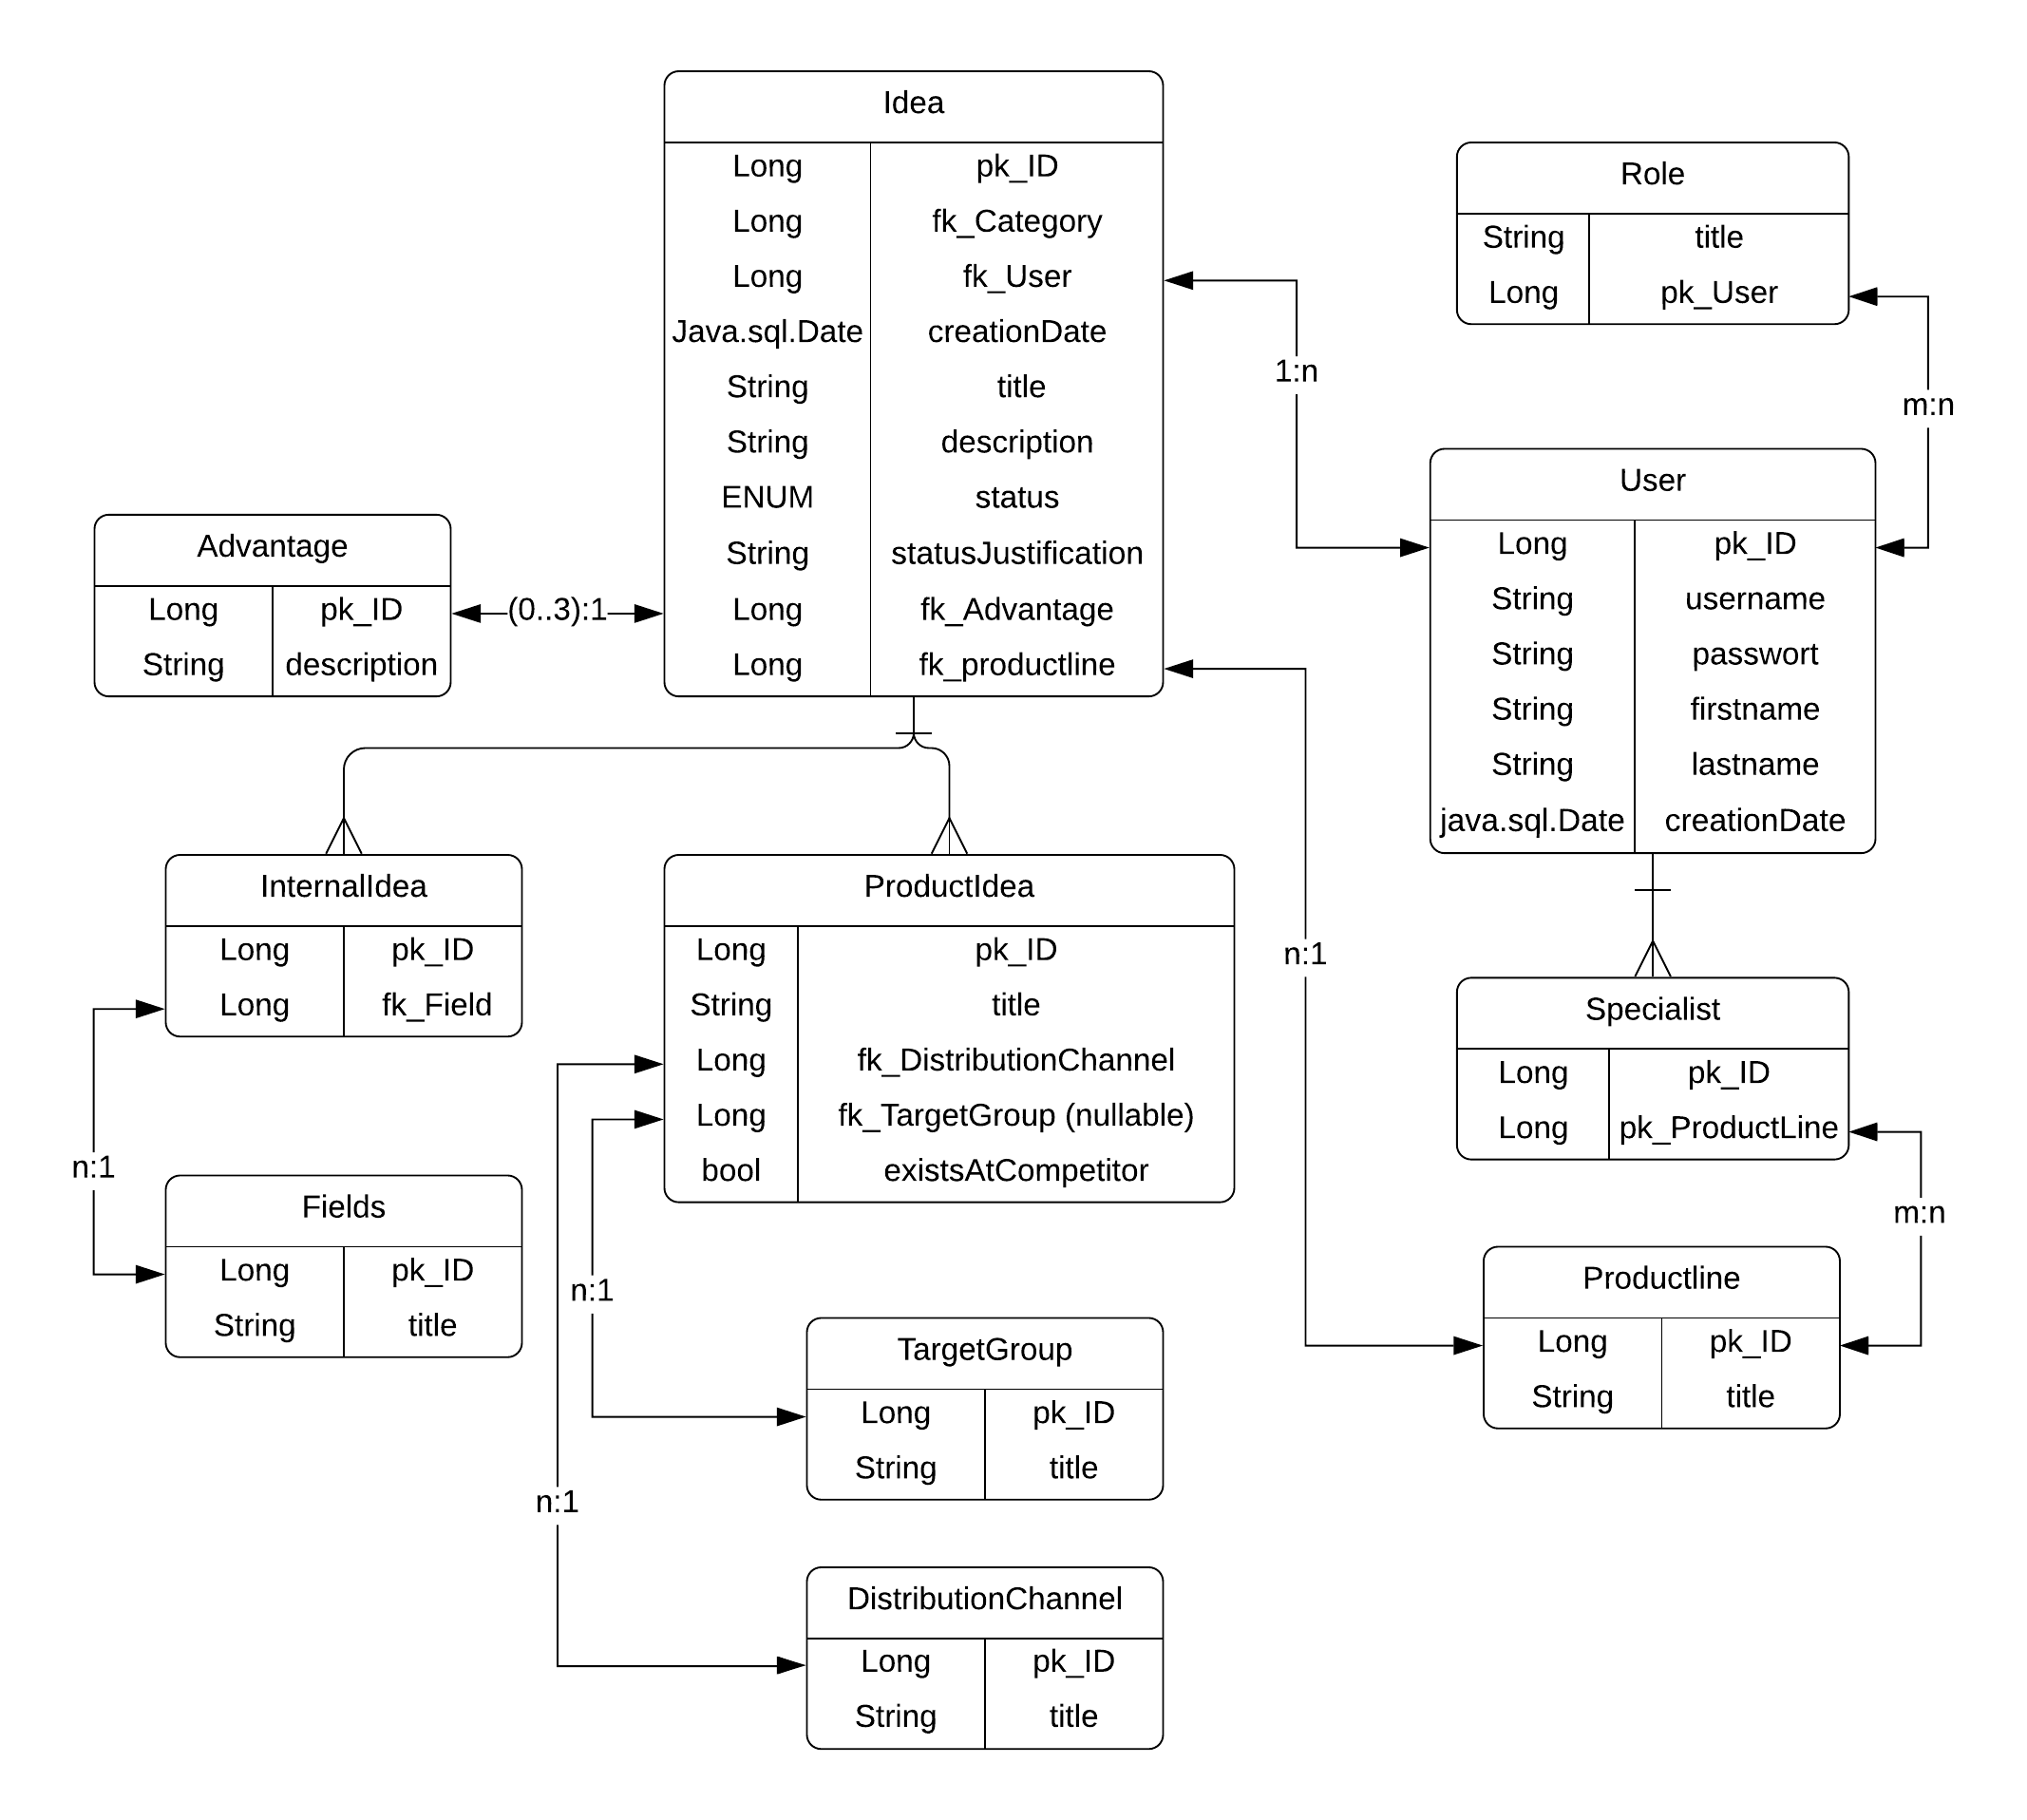
\includegraphics[width=1\textwidth]{img/erd.png}\\
        \source{Eigene Darstellung}
        \label{fig:erd}
    \end{minipage}
\end{figure}

Dieses Diagramm wurde im Programm in der Datenbank umgesetzt. Im Folgenden werden einige Design-Entscheidungen erläutert.\\
\textbf{Zuordnung von Fachspezialisten und Ideen}\\
Um die automatische Zuordnung von Fachspezialisten zu Ideen umzusetzen, haben wir die Produktsparte als Zuordnungskriterium herangezogen.
Die Klasse des Fachspezialisten erbt vom der Klasse des Benutzers mit der zusätzlichen Eigenschaft, dass ihm eine oder mehrere Produktlinien zugewiesen sind.
Einer Produktsparte können mehrere Fachspezialisten zugeordnet sein. Mit dieser m:n-Beziehung erreicht das Programm die größtmögliche Flexibilität.
Jeder Idee (Intern und Produkt) ist eine Produktsparte zugeordnet. Aus den Projektanforderungen ergeben sich mehrere Produktsparten, die bei der Auslieferung bereits vorhanden sind.
Da interne Ideen gemäß der Anforderungen keine Produktsparte besitzen, bekommen Sie die dem Benutzer verborgene Produktsparte \glqq{}INTERNAL\grqq{} zugewiesen. Diese ermöglicht für interne Ideen dieselbe Logik zu verwenden.
Durch diese Umsetzung ist auch eine Erweiterung um weitere Ideenkategorien ohne Änderungen am übrigen Programm möglich.\\
\textbf{Umsetzung von Status}\\
Wir haben uns dagegen entschieden, den Status in eine eigene Entität im Sinne des ERD auszulagern.
Erweiterungen und Änderungen der Status im Echtbetrieb erfordern dann zwar unter Umständen an einigen Stellen Änderungen in der Programmlogik aber die enum bieten insgesamt Performancevorteile gegenüber der Auslagerung als vollwertige Entität und sind leichter im Code umzusetzen.\\
\textbf{Vererbung von Ideen zu interne und Produktidee}\\
Das Anlegen von Klassen mit Vererbung (wie im Projekt bei Ideen und Usern) kann in relationalen Datenbanken zu zwei Schwierigkeiten führen:
\begin{enumerate}
    \item {Lese- und Speicherzugriffe betreffen mehrere Tabellen und erfordern Joins. Das kann zu unübersichtlichen Strukturen und SQL-Kommandos sowie zu geringerer Performance führen}
    \item {Nicht-polymorphe Abfragen (z.B. Namen/Preise nur der Getraenke) sind umständlich (z.B. Unterscheidung per Diskriminator)\footnote{vgl. \cite{Horn2007}}}
\end{enumerate}
Durch die Verwendung von Hibernate mit seiner nativen Java-Integration und die Vermeidung von hardcodeten SQL-Statements im Code, fallen diese Punkte kaum ins Gewicht. Die Struktur der Vererbung ermöglicht es darüber hinaus sogar weitere Kategorien von Ideen anzulegen.




    %!TEX root = ../Thesis.tex
%! Author = PR
%! Date = 27.05.2020


\section{Projekt-Architektur \textcolor{blue}{[Philipp Röring]}}

In \cref{fig:root-ordner} ist die grobe Ordnerstruktur des Quellcodes dargestellt.

\begin{figure}[htb]
    \centering
    \begin{minipage}[t]{1\textwidth}
        \caption{Grobe Ordnerstruktur}
        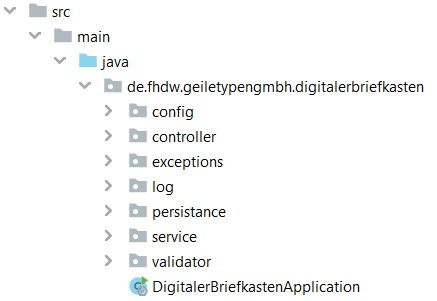
\includegraphics[width=0.5\textwidth]{img/Projekt-root-ordner.png}\\
        \source{Eigene Darstellung}
        \label{fig:root-ordner}
    \end{minipage}
\end{figure}

In dem Projektordner befinden sich der Unterordner \textit{src/main/java/de/fhdw/geiletypengmbh/digitalerbriefkasten}. In diesem
befindet sich der erstellte Quelltext. Die Unterordner (Packages) dessen werden folgend grob erklärt.
\begin{itemize}
    \item config
    \subitem Hierin ist die SecurityConfig der Anwendung enthalten.
    \item controller
    \subitem Hierin liegen die Controller. Diese stellen die erreichbaren Endpunkte für die Benutzeroberfläche sowie die REST-API zur Verfügung.
    \item exceptions
    \subitem Hierin sind eigene Exceptions. Diese werden an die Benutzeroberfläche im Fehlerfall weitergeleitet. Ein Beispiel dafür ist die "IdeaNotFoundException".
    \item log
    \subitem Hierin liegen alle Klassen, die zum Logging von Ereignissen dienen.
    \item persistance
    \subitem Das Package persistance dient zum Speichern der Daten (Objekte bzw. Entities) in der Datenbank. Es ist untergliedert
    in die packages
    \begin{itemize}
        \item model
        \subitem Hierin liegen die Datenklassen (Entities). Sie entsprechen dem ER-Diagramm.
        \item repo
        \subitem Hierin liegen die Repositories. Sie dienen zum Lesen, Schreiben, etc. der Datenklassen in die Datenbank.
    \end{itemize}
    \item service
    \subitem Hierin liegen die Services. Sie dienen als Abstraktionsschicht über den Repositories. Damit kann zusätzliche Logik z.B. vor dem Speichern einer Entität implementiert werden. Auch Hilfsmethoden befinden sich in den Services.
    \item validator
    \subitem Hierin liegt die Validationsklasse für die Benutzerstellung. Sie enthält Prüfungen, wie z.B. ob das Passwort lang genug ist.
\end{itemize}
Darüber hinaus befindet sich in dem Package noch die Hauptklasse der Anwendung \textit{DigitalerBriefkastenApplication}, durch welche sie gestartet wird.
\newline
Neben \textit{src/main/java} existiert auch der Ordner \textit{src/main/resources}. In diesem sind die Komponenten für die Weboberfläche der Anwendung enhalten.
In \cref{fig:resources-ordner} wird die Struktur von resources dargestellt.

\begin{figure}[htb]
    \centering
    \begin{minipage}[H]{1\textwidth}
        \caption{Grobe Ordnerstruktur}
        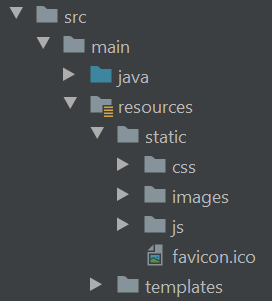
\includegraphics[width=0.5\textwidth]{img/resources-ordner.png}\\
        \source{Eigene Darstellung}
        \label{fig:resources-ordner}
    \end{minipage}
\end{figure}

Der Unterordner static beinhaltet css-, Bild- und JavaScript-Dateien. In Templates befinden sich die HTML Dateien.

\subsection{Klassendiagramm}
In \cref{fig:advantage-klassendiagramm} wird die Architektur beispielhaft erklärt:

\begin{figure}[htb]
    \centering
    \begin{minipage}[H]{1\textwidth}
        \caption{Klassendiagramm Advantage}
        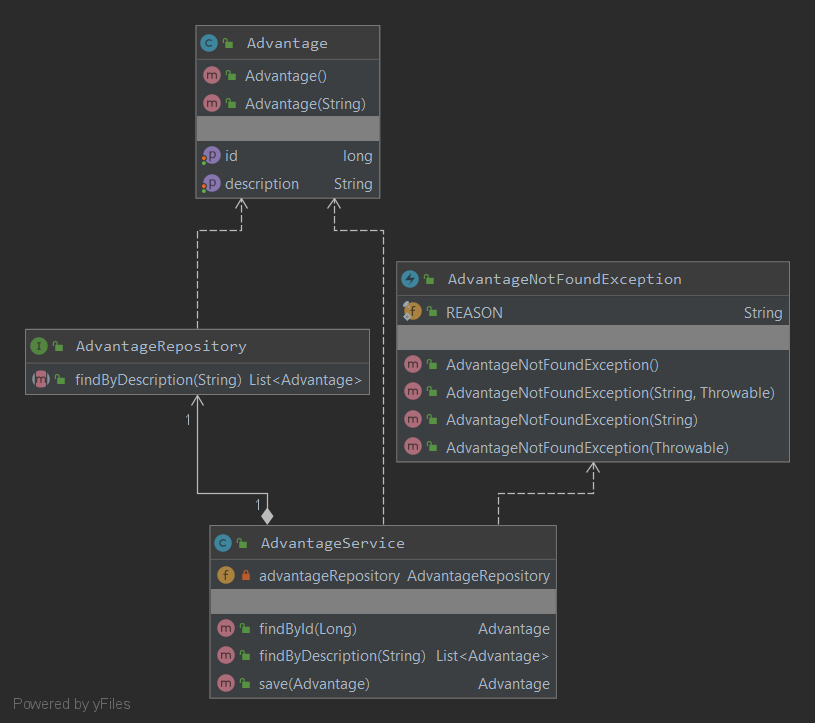
\includegraphics[width=0.75\textwidth]{img/advantage-klassendiagramm.png}\\
        \source{Eigene Darstellung}
        \label{fig:advantage-klassendiagramm}
    \end{minipage}
\end{figure}

Die Klasse \textit{Advantage} stellt die Entität dar, welche die gesamte Anwendung durchläuft.
Das \textit{AdvantageRepository} ist eine Erweiterung des \textit{JPARepositories} und dient somit zur Interaktion mit der Datenbank und Advantage-Objekten.
Darauf aufbauende Logik wird in dem \textit{AdvantageService} implementiert. Dieser wirft z.B. eine \textit{AdvantageNotFoundException} in der
Methode \textit{findById()}, wenn keine Advantage in der Datenbank gefunden wird.
\\
Auf ein Klassendiagramm der gesamten Anwendung wurde verzichtet, da es zu unüberischtlich ist.
In Anhang \ref{Anhang:Klassendiagramme} sind Klassendiagramme des Models zu finden, die dem ER-Diagramm entsprechen.





    %!TEX root = ../Thesis.tex
%! Author = PR
%! Date = 27.05.2020


\section{Abläufe \textcolor{blue}{[Philipp Röring]}}

In \cref{fig:digitaler-briefkasten-pap} wird der grobe Ablauf der Anwendung in Form eines Programmablaufplans skizziert.
Dabei sollte beachtet werden, dass Maven nur während der Entwicklung der Anwendung relevant ist und nicht in der kompilierten
Anwendung enthalten ist.

\begin{figure}[h!!]
    \centering
    \begin{minipage}[t]{0.7\textwidth}
        \caption{Ablauf der Anwendung}
        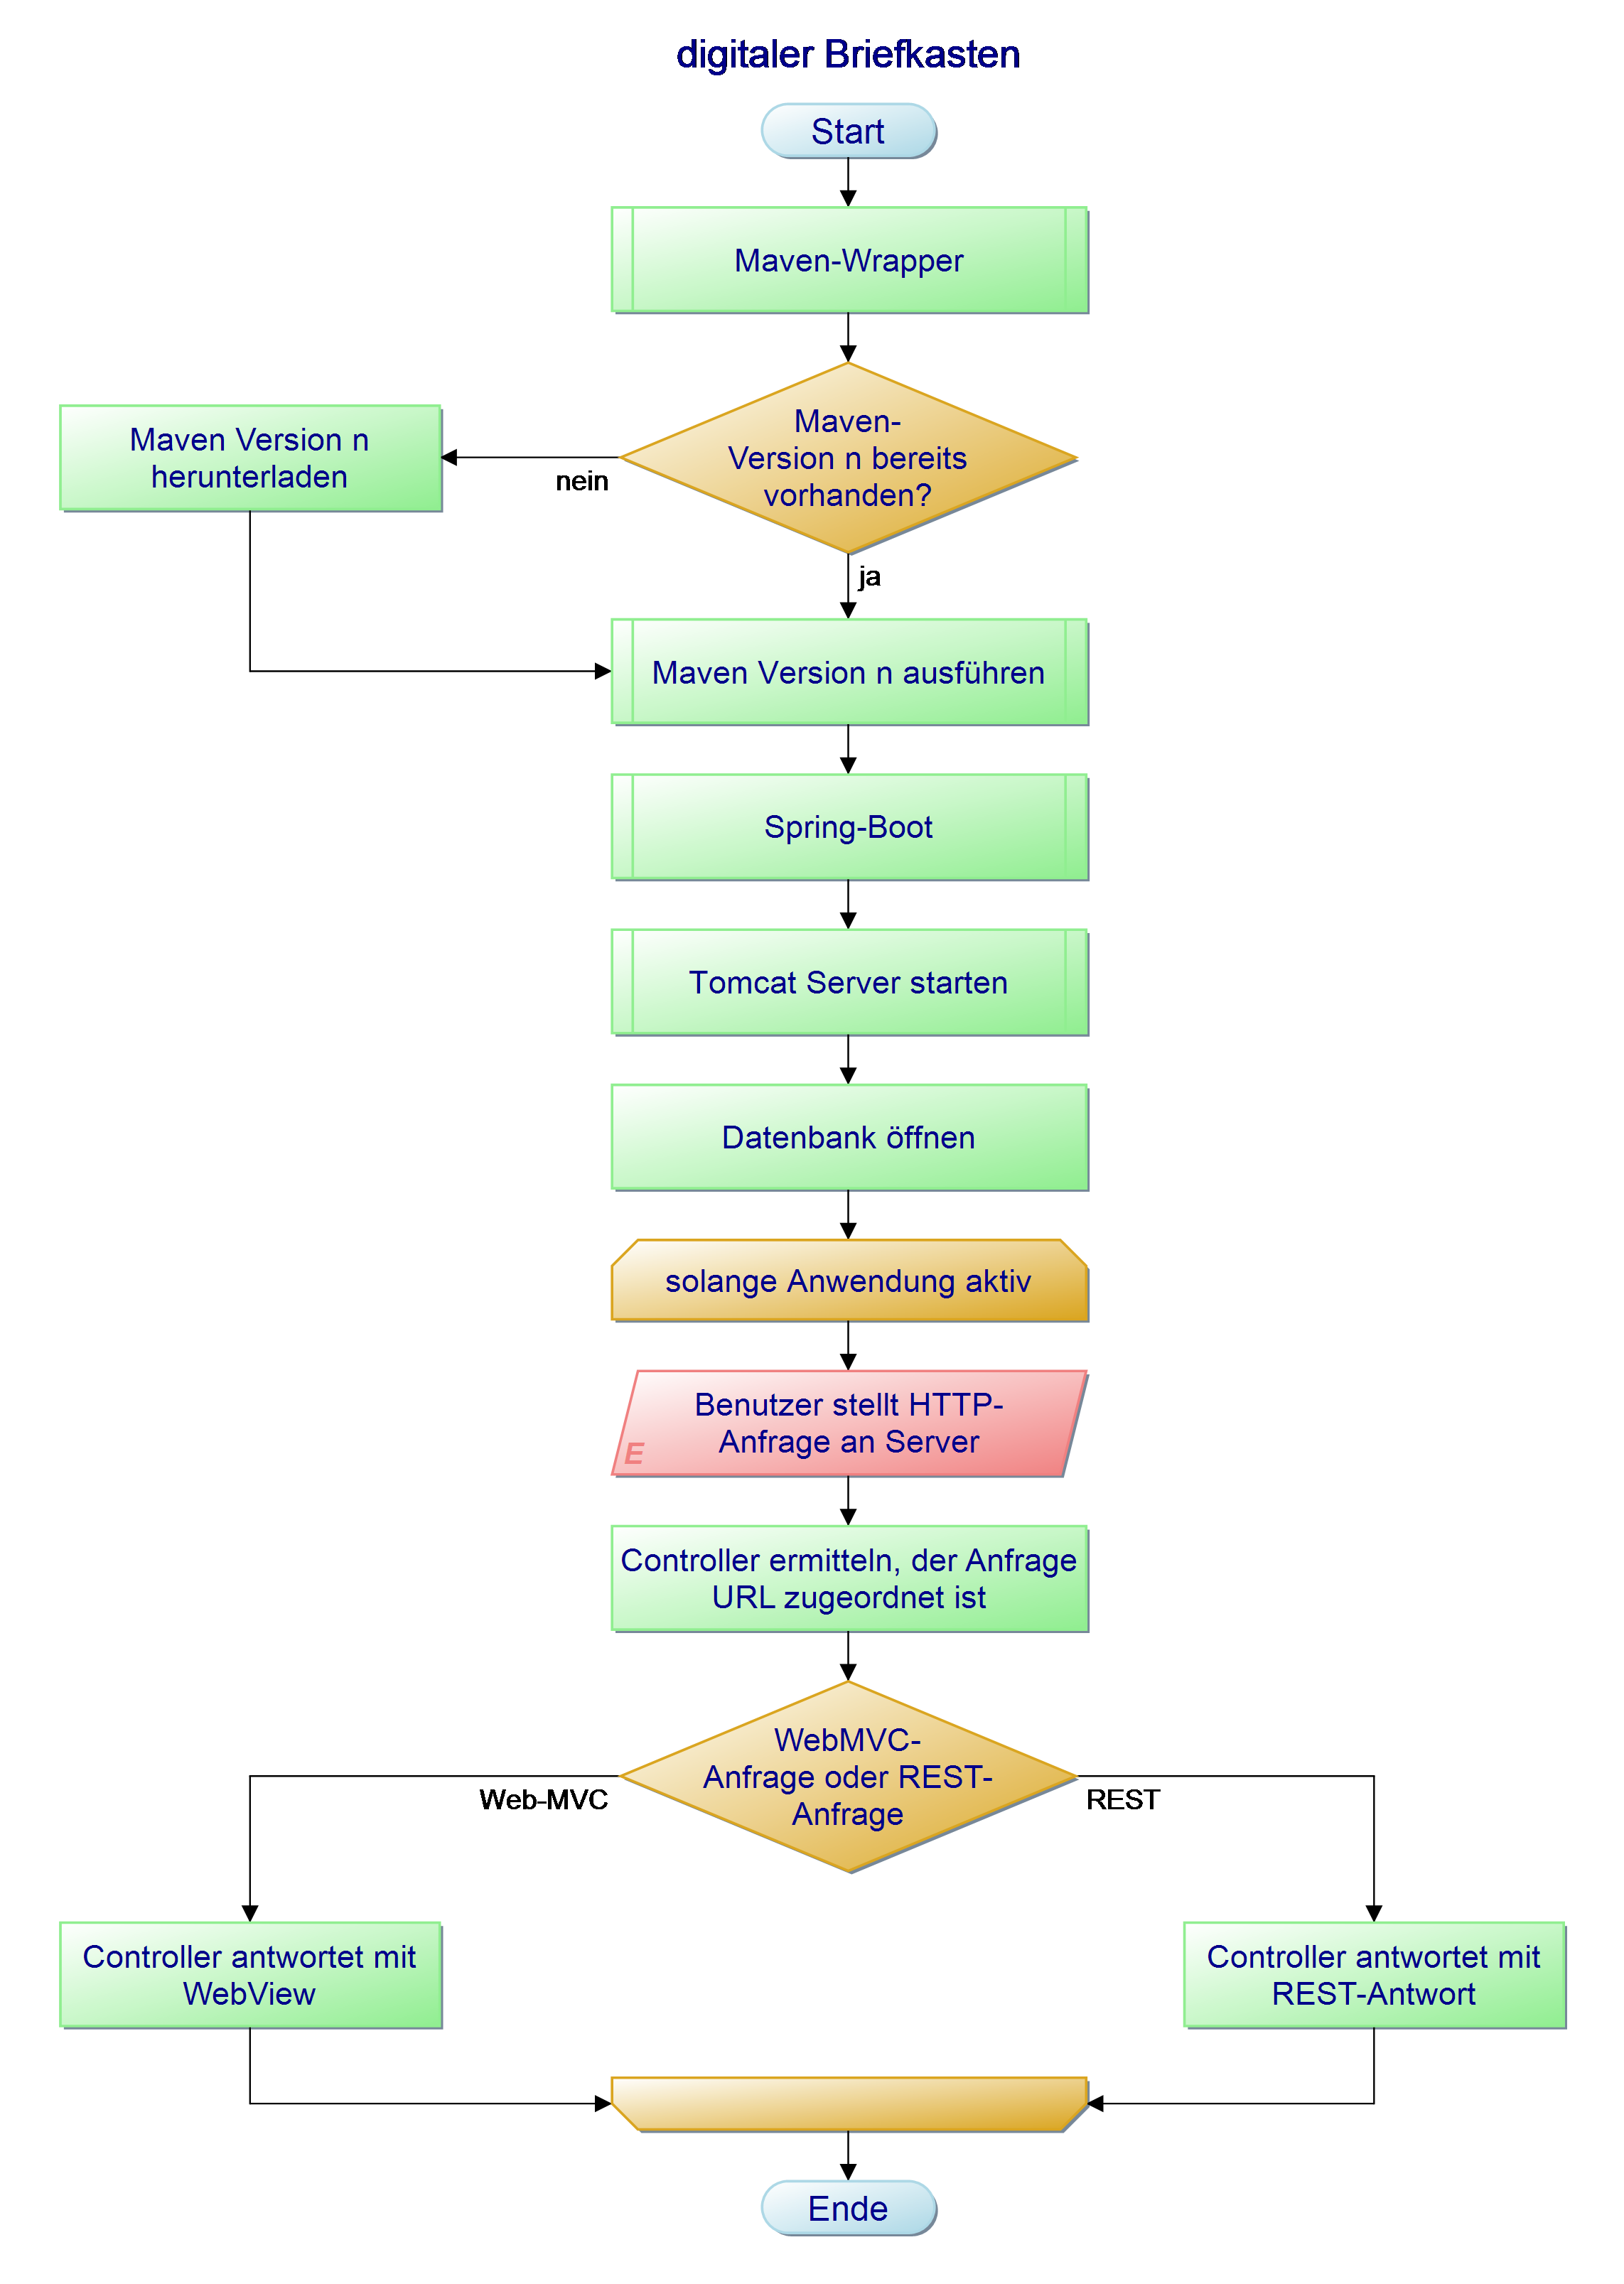
\includegraphics[width=1\textwidth]{img/digitaler-Briefkasten-pap.png}\\
        \source{Eigene Darstellung}
        \label{fig:digitaler-briefkasten-pap}
    \end{minipage}
\end{figure}









    %!TEX root = ../Thesis.tex
%! Author = PR
%! Date = 27.05.2020


\section{Schnittstellen \textcolor{blue}{[Philipp Röring]}}

Die Anwendung ist über eine REST-API erreichbar. Alle Antworten sind im JSON-Format.

\subsection{Schnittstellenbeschreibung REST-API}
Die Schnittstelle stellt folgende Services bereit:
\begin{itemize}
    \item HTTP-Methode: GET
    \subitem Relativer Pfad: \textit{/api/ideas/}
    \subitem Antwort: Array, das alle Ideen (Proukt-/ Interne Ideen) beinhaltet.
    \subitem Beispielantwort: siehe Anhang \ref{Anhang:Schnittstellen1}
\end{itemize}

\begin{itemize}
    \item HTTP-Methode: GET
    \subitem Relativer Pfad: \textit{/api/ideas/\{id\}}
    \subitem Antwort: Idee (Proukt-/ Interne Idee) in JSON-Format
    \subitem Beispielantwort: siehe Anhang \ref{Anhang:Schnittstellen2}
\end{itemize}

\begin{itemize}
    \item HTTP-Methode: GET
    \subitem Relativer Pfad: \textit{/api/ideas/title/\{title\}}
    \subitem Antwort: Idee (Proukt-/ Interne Idee) in JSON-Format
    \subitem Beispielantwort: siehe Anhang \ref{Anhang:Schnittstellen2}
\end{itemize}

\begin{itemize}
    \item HTTP-Methode: GET
    \subitem Relativer Pfad: \textit{/api/ideas/submitted}
    \subitem Antwort: Array, das alle Ideen (Proukt-/ Interne Ideen), die veröffentlicht sind, beinhaltet.
    \subitem Beispielantwort: siehe Anhang \ref{Anhang:Schnittstellen1}
\end{itemize}

\begin{itemize}
    \item HTTP-Methode: POST
    \subitem Relativer Pfad: \textit{/api/ideas/}
    \subitem Mitzugebener HTTP-Body: Idee in JSON-Format (Syntax siehe GET-Methoden)
    \subitem Bei Erfolg
    \subsubitem HTTP-Status 201 im HTTP-Header, sowie die erstellte Idee als Json im HTTP-Body
    \subitem Bei Fehler
    \subsubitem Fehlerrückmeldung
    \subitem Beispielantwort: siehe Anhang \ref{Anhang:Schnittstellen2}
\end{itemize}

\begin{itemize}
    \item HTTP-Methode: DELETE
    \subitem Relativer Pfad: \textit{/api/ideas/\{id\}}
    \subitem Antwort: HTTP-Status 200 bei Erfolg, ansonsten Fehlerrückmeldung
\end{itemize}

\begin{itemize}
    \item HTTP-Methode: PUT
    \subitem Relativer Pfad: \textit{/api/ideas/\{id\}}
    \subitem Mitzugebener HTTP-Body: Idee in JSON-Format (Syntax siehe GET-Methoden)
    \subitem Antwort: HTTP-Status 200 bei Erfolg, ansonsten Fehlerrückmeldung
\end{itemize}

\begin{itemize}
    \item Fehlerrückmeldung der API
    \subitem Beispielantwort:
    \begin{verbatim}
    {
        "timestamp": "2020-05-28 12:20:59.386",
        "status": 404,
        "error": "Not Found",
        "message": "Keine entsprechende Idee gefunden",
        "path": "/api/ideas/111"
    }
    \end{verbatim}
    \subitem Der Status der Antwort entspricht dem Status des HTTP-Header der Antwort.
\end{itemize}

\subsection{Login}
Um die GET- \textit{/api/ideas/} sowie die POST-, DELETE- und PUT- Aufrufe der API nutzen zu können, muss sich mit einem Benutzer der Rolle \textit{API\_USER} angemeldet werden.
Dies wird hier nicht genauer spezifiert, da es keine Anforderung war.
Die Funktionalität wurde aber bereits in der Basis für zukünftige Erweiterungen hinzugefügt und kann mit einem REST-Client getestet werden.
Ein \textit{API\_USER} kann mit Hilfe des Skripts \textit{HelperScriptNoTests} erstellt werden.
Die restlichen GET-Methoden können ohne Authentifizierung aufgerufen werden. Diese entsprechen den Ideen, die auch in der Benutzeroberfläche ohne Anmeldung angesehen werden können.

\subsection{Webschnittstelle}
Die restlichen Schnittstellen, die von der Benutzeroberfläche verwendet werden, verwenden das Format \textit{application/x-www-form-urlencoded}.
Jenes Format ermöglicht die native Verwendung von HTML-Forms ohne die Formulardaten per JavaScript umformen zu müssen.
Um diese Aufrufe testen zu können, können die Entwickleroptionen eines Webbrowsers oder ein REST-Client verwendet werden.
Dazu muss in den HTTP-Header des Requests der Cookie \textit{JSESSIONID} und das \textit{X-CSRF-TOKEN} eingefügt werden.
Diese können dem Browser in den Entwickleroptionen nach einem Login entnommen werden.

    %%%%%%%%% JULIUS %%%%%%%%%%%%%%%
    %!TEX root = ../Thesis.tex
\section{Security  \textcolor{blue}{[Julius Figge]}}
\label{Security}

Die Security der Anwendung wird durch mehrere Bestandteile sichergestellt, diese lassen sich in aktive und passive Elemente unterteilen.\footnote{Zu beachten ist, dass wir das Programm unter der Prämisse entwickelt haben, dass im Livebetrieb eine zusätzliche SSL-Verschlüsselung für den Traffic genutzt wird.} 
\subsection{Aktive Security Bestandteile}
Zuerst ist der Login sowie die Registrierung abgesichert. Nutzer müssen ihr Passwort mit mindestens 8 Zeichen wählen. Dieses wird im Backend, inklusive Salt, gehashed gespeichert. Hierzu benutzen wir BCrypt als Passwort Encoder. Diesen verwenden wir mit einer Stärke von 10, das bietet für uns die beste Balance zwischen Sicherheit und Performance. Mit dem Login bekommen Nutzer einen Cookie, in Form einer JSession ID, mit dem sie sich in weiteren Requests authentifizieren und über den sie identifiziert werden können.\\
Der nächste Bestandteil ist die URL-Zugriffskontrolle in der Klasse \enquote{SecurityConfig} im Package \enquote{config}. In dieser wird festgelegt welche Requests durch Spring Security zugelassen werden. Nicht authentifizierte Nutzer haben hier nur Zugriff auf statische Elemente (wie z.B. Grafiken, Javascript und CSS), die Registrierung und die Ideenansicht.
Authentifizierte Nutzer werden anhand ihrer Rolle unterschieden, welche im Backend überprüft wird. Nutzer, Spezialisten und Administratoren können nur auf die jeweils für sie relevanten Seiten zugreifen.
Der durch Spring Security erstellte JSession-Cookie wird beim ausloggen invalidiert und gelöscht.\\
Darüber hinaus ist die Anwendung so konfiguriert, dass ein automatischer Session Timeout nach 15 Minuten erfolgt, auch hierbei wird die Session invalidiert.\\
Außerdem werden alle Abfragen durch das Backend geprüft. An relevanten Stellen wird in den jeweiligen Controllern bereits vor der Bearbeitung des Requests die Rolle des aktuellen Users überprüft. Damit wird sichergestellt, dass Funktionen die insbesondere dem Administrator oder Spezialisten vorbehalten sind, nur durch diese durchgeführt werden können. \\
Außerdem werden übertragene Informationen in den bearbeitenden Services um die Berechtigung diese anzufragen, zu verändern oder zu speichern geprüft.\\
Durch diese Kontrolle an mehreren Stellen erreichen wir es zu kontrollieren und sicherzustellen welche Art von Requests ( un-, authentifiziert), welcher User, welcher Rolle, welche Daten wie verwenden (lesen, bearbeiten, schreiben) dürfen.\\

\subsection{Passive Security Bestandteile}
Zu den passiven Bestandteilen gehört das Loggen von Anmeldeversuchen, Anmeldung, Registrierung, und Abmeldung vom System.\footnote{Das Loggen von Session Timeouts konnte aufgrund von Komplikationen zum Abgabezeitpunkt nicht fertiggestellt werden.}
Dies wird duch mehrere Klassen im Package \enquote{log} sichergestellt. Diese implementieren einen jeweiligen Application-Listener, beispielhaft für den fehlerhaften Login der ApplicationListener \texttt{AuthenticationFailureBadCredentialsEvent}. Beim auftreten eines passenden Applicationevents wird mit Hilfe eines Loggers, den \enquote{slf4j} bereitstellt der aktuelle Zeitstempel sowie Nutzername und IP-Adresse geloggt.
Hierbei ist anzumerken, dass die Logs zusätzlich außerhalb der Konsole in eine Datei geschrieben werden. Diese ist auf 5Mb begrenzt und rotiert oberhalb dieser Grenze automatisch. 
Zudem sind die zu schreibenden Logs eingeschränkt. 
Damit stellen wir sicher, dass nur relevante Informationen festgehalten werden und diese auch unabhängig vom Programm zur Auswertung zur Verfügung stehen.
Des weiteren sind Fehlermeldungen eingeschränkt um nicht aus versehen Informationen durchsickern zu lassen. Beispielhaft zeigt der Login ausschließlich eine Fehlermeldung bei fehlerhaften Daten an - jedoch nicht ob der Nutzername oder das Passwort falsch war.
\textcolor{red}{Darüber hinaus werden Exceptions gefiltert und nur ausgewählte (respektive unsere eigenen) auf der Error-Seite angezeigt. Damit stellen wir sicher, dass nicht ausversehen Exceptions, Stacktraces oder Debug-Logs an das Frontend gelangen und für den Nutzer sichtbar sein könnten.}


    %!TEX root = ../Thesis.tex


\section{Test}
\subsection{manuelle-\enquote{Klicktests}}

Zur Überprüfung der \enquote{GUI} sollen manuelle Klicktests durchgeführt werden.
Diese sollen dokumentiert werden um Fehler möglichst gezielt beheben zu können.\\

\subsubsection*{Zu notierende Informationen}
\begin{itemize}
\item Revision (Git Commit Hash, Datum) sowie Branch
\item Betriebssystem
\item Browser (inklusive Build)
\item Bildschirmauflösung, Fenstergröße (nach Möglichkeit)
\item auftretende Fehler (inklusive Screenshots)
\end{itemize}

\subsubsection*{Testvorbereitung}
\begin{enumerate}
    \item Zum Testen wird der neueste Stand des master-Branches verwendet. 
	\item Hierzu ist zunächst die Datenbank zu löschen und mit Hilfe der in \enquote{HelperScriptsNoTests} 		vorhandenen Tests zu füllen.
	\item Der Code soll kompiliert werden und die entstandene \enquote{Jar}-Datei ausgeführt werden.
    \item Nach Möglichkeit soll der Test auf mehreren Browsern ausgeführt werden. Hierbei ist zu beachten, dass alle Addons zu deaktivieren sind, um eventuelle Komplikationen auszuschließen.
    \item Nachdem diese Voraussetzung geschaffen ist, sind die Tests durchzuführen und die obigen Informationen zu notieren.
\end{enumerate}

\subsubsection*{Testdurchführung}
\begin{enumerate}
\item \textbf{Registrieren} eines neuen Nutzers
	\subitem Bereits bestehenden Nutzernamen verwenden (admin)
	\subitem Mit nicht den Richtlinien entsprechendem Nutzernamen
	\subitem Mit nicht den Richtlinien entsprechendem Passwort
	\subitem Mit nicht übereinstimmenden Passwörtern
	\subitem Korrektes Passwort
\item \textbf{Ausloggen} aus dem Account
\item \textbf{Einloggen} in den erstellten Account
	\subitem Mit falschem Nutzernamen
	\subitem Mit falschem Passwort
	\subitem Mit richtigem Passwort
\item \textbf{Erstellen} von beispielhaften \textbf{Ideen}
	\subitem Erstellen einer \enquote{internen Idee}
	\subitem Erstellen einer \enquote{Projekt-Idee}
	\subitem Erstellen einer beliebigen Idee mit fehlerhaften / fehlenden Werten
	\subitem Bereits bestehenden Namen verwenden
\item Ideenübersicht \textbf{prüfen}
\item \textbf{Bearbeiten} der Werte beider \textbf{Ideen}
\item Ideenübersicht \textbf{prüfen}
	\subitem Filtern der Tabelle nicht eingereichter Ideen nach nach allen Spalten (und Typ)
\item \textbf{Einreichen} beider \textbf{Ideen} zur Bearbeitung
\item Ideenübersicht \textbf{prüfen}
\item \textbf{Ausloggen}
\item \textbf{Ansicht der Ideen} als nicht eingeloggter Nutzer
	\subitem Filtern der Ideen als nicht eingeloggter Nutzer
\item \textbf{Einloggen als Spezialist} für \enquote{internen Idee}
\item \textbf{Übersicht} zu entscheidender Ideen \textbf{ansehen}
	\subitem Übersicht zu entscheidender Ideen filtern
	\subitem Entscheiden über Idee mit fehlerhafter Eingabe
	\subitem Verschieben der Idee in Ideenspeicher
\item Ideenübersicht \textbf{prüfen}
\item \textbf{Ausloggen}
\item \textbf{Einloggen als Spezialist} für vorgehend eingereichte \enquote{Projekt-Idee}
\item Idee aus Ideenspeicher \textbf{annehmen}
\item Idee aus Entscheidungsübersicht \textbf{bewerten}
\item Ideenübersicht \textbf{prüfen}
\item \textbf{Ausloggen}
\item \textbf{Einloggen} als \enquote{admin}
\item Existierende \textbf{User prüfen}
\item Alle möglichen \textbf{anzulegenden Felder durchgehen}
 \subitem Zuerst Bereits bestehenden Namen beim anlegen verwenden
 \subitem Danach neuen Namen verwenden
\item \textbf{Ausloggen}
\item Fertig!
\end{enumerate}


    %!TEX root = ../Thesis.tex

\section{Use-Cases}

Im nachfolgenden sind die Use-Cases des Programm dargestellt.
Diese sind den Projektvorgaben entnommen.\footnote{Vgl. \cite{Vorgaben2020}}

\begin{figure}[hbt]\label{Uploadvert}
\centering
\begin{minipage}[t]{1\textwidth} 
\caption{Use-Case Diagramm} 
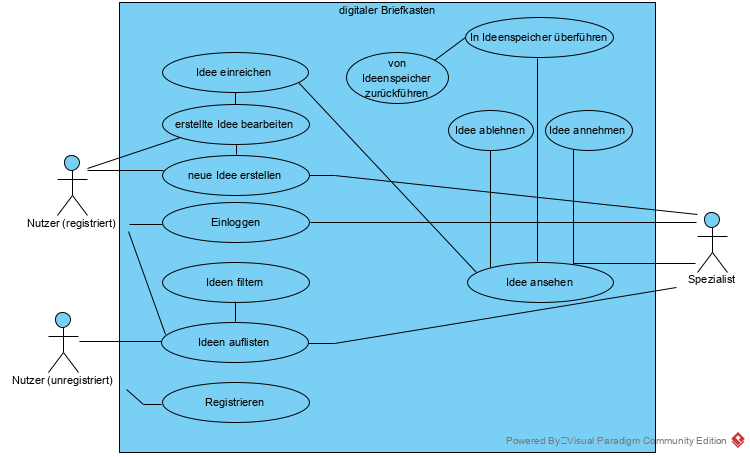
\includegraphics[width=1\textwidth]{img/createAnAccountWithSpamMailAccountYouSucker.png}\\
\source{Eigene Darstellung} 
\label{fig:Use-Case}
\end{minipage}
\end{figure}

Für das Use-Case Diagramm sind drei Rollen von Relevanz. 
Zuerst der \texttt{unregistrierte Nutzer}, welche die Sicht des Programmes für die Öffentlichkeit repräsentiert.
Desweiteren der \texttt{eingeloggte Nutzer} der mehr Möglichkeiten hat, hierzu gehört auch der\texttt{Administrator}. 
Dieser hat über die Möglichkeiten des Nutzers weitere administrative Rechte.\footnote{Der Admin ist als eigener Use-Case im Anhang dargestellt. Siehe Anhang \ref{Anhang-Admin} auf S.\pageref{Anhang-Admin}}
Jedoch besitzt er nicht die Rechte der dritten Rolle des \texttt{Spezialisten}.\\

Die Use-Cases lassen sich in zwei \enquote{Kern}-Kategorien unterteilen.
Das sind zum einen die \texttt{Account} bezogenen Use-Cases.\\
Hierzu gehören der Vorgang des Einloggens sowie der Registrierung.
Zu diesen ist anzumerken, dass Spezialisten sich lediglich einloggen können. 
Durch ihre administrative Rolle werden diese durch den Administrator angelegt.\\
Zum anderen ist der zweite Use-Case die \texttt{Erstellung und Bewertung von Ideen}.\\
Eingereichte Ideen lassen sich durch alle Nutzer jeder Rolle einsehen und filtern. Darüber hinaus haben alle eingeloggten Nutzer die Möglichkeit Ideen zu erstellen, zu bearbeiten und zur Bewertung einzureichen.\\
Diese eingereichten Ideen werden durch Spezialisten bewertet oder gespeichert.

Desweiteren exisitiert die Möglichkeit für alle Nutzer dem Administrator der Plattform über ein Kontaktformular Nachrichten zu senden.\footnote{Das zugehörige Use-Case Diagramm findet sich im Anhang \ref{Anhang-Kontakt} auf S.\pageref{Anhang-Kontakt}}

    %!TEX root = ../Thesis.tex


\section{GUI-Konzept \textcolor{blue}{[Julius Figge]}}

Wir haben uns entschieden, statt eines GUI-Mockups unser GUI-Konzept direkt im Prototypen mit auszuliefern.
Das lässt sich durch mehrere Punkte begründen.
Zuerst hatten wir zum Zeitpunkt der ersten Präsentation bereits einen funktionierenden Prototypen und konnten diesen direkt mit dem GUI-Konzept ausstatten. Dadurch hatten wir nicht nur ein Mockup sondern konnten bereits mit der GUI interagieren.
Des weiteren hatten wir dadurch die Möglichkeit die Zeit für die Erstellung eines Konzeptes direkt in die Entwicklung funktionierender GUI zu stecken.

Die GUI wurde unter Nutzung von Bootstrap 4 in Kombination mit Font-Awesome für die Icons entwickelt.
Dadurch war es uns mögliche eine konsistente, verständliche und klare Oberfläche zu entwickeln.
Hierbei haben wir uns darauf konzentriert \enquote{eine klare Linie zu fahren}. Alle Seiten werden auf weißem Hintergrund dargestellt. Buttons und Informationen sind generell in grau ( beziehungsweise Schwarz) gehalten.
Abweichend hiervon treten Farben nur auf um die Aufmerksamkeit des Nutzers auf sich zu ziehen oder um Hinweise hervorzuheben. Diese Farben sind in \cref{fig:Farbmuster} abgebildet. Die Verwendung wird im weiteren näher erläutert.

\begin{figure}[hbt]
    \centering
    \begin{minipage}[t]{1\textwidth}
        \caption{Farben Konzept}
        \includegraphics[width=0.5\textwidth]{img/Farbmuster.png}\\
        \source{Eigene Darstellung}
        \label{fig:farbmuster}
    \end{minipage}
\end{figure}


Grundlegend sind die Elemente der Anwendung zentriert wie im weiteren zu sehen. Damit erreichen wir in Kombination mit der Nutzung von Bootstrap eine nahezu 100 prozentige Kompatibilität zu mobilen Endgeräten.\footnote{Hierbei ist jedoch anzumerken, dass dieses Feature nicht gefordert war und somit auch nicht weitergehend getestet wurde. Allerdings sind bereits die Voraussetzungen für eine mögliche Erweiterung der Anwendung geschaffen.}

Grundlegende Elemente dieses Konzeptes sind zum einen der Login-Screen (Siehe \cref{fig:Login} im Anhang auf S.\pageref{fig:Login}).
In diesem Screenshot ist auch das Logo der Anwendung zu sehen welches ebenfalls in den typischen Farben gehalten wurde. Dieses soll der Anwendung einen Wiedererkennungswert geben durch seine gleichzeitig humorvolle als auch simple Darstellung.

Die zweite zentrale Komponente des Konzeptes ist die Übersicht aller Ideen (Siehe \cref{fig:ideen}).
Auffallend ist hier die Gliederung der Ideen in Tabellen. Bereits zu diesem Zeitpunkt war geplant die Ideen nach Typ zu gliedern und in einer Übersicht mit ihren wichtigsten Eigenschaften darzustellen.
Zu diesem Zeitpunkt noch per Klick\footnote{Diese Funktionalität wurde im weiteren durch ein Rechtsklick Menü erweitert (Siehe \ref{GUI-Umsetzung} S.\pageref{GUI-Umsetzung}).}, sollte es möglich sein die Idee im Detail inklusive aller Informationen darzustellen. Diese Entscheidung begründest sich damit das Gleichgewicht zwischen der verfügbaren Information auf einer Seitenansicht und der Übersichtlichkeit zu wahren.
Darüber hinaus findet sich auch hier die Farbgestaltung wieder. Grundsätzlich ist die Oberfläche Monochrom gehalten. Icons dienen der schnelleren Identifikation der verschiedenen Tabellen und der Übersichtlichkeit. Farbakzente sind zum einen zur Führung der Nutzer gedacht, siehe beispielhaft in dem Hyperlink auf den Ersteller der Ideen\footnote{Dieser Hyperlink stand beispielhaft für die Weiterleitung auf eine Detailseite auf der Tabellensicht.}. Zum anderen sind diese in den Status der Ideen mit einbezogen, hierdurch lässt sich erheblich schneller ein Überblick verschaffen.

\begin{figure}[hbt]
    \centering
    \begin{minipage}[t]{1\textwidth}
        \caption{Ideen Konzept}
        \includegraphics[width=1\textwidth]{img/ideen-Konzept.png}\\
        \source{Eigene Darstellung}
        \label{fig:ideen}
    \end{minipage}
\end{figure}

Ein weiterer relevanter Punkt der sich beispielhaft in dieser Abbildung (Siehe \cref{fig:ideen}) findet ist die Navigationsleiste. Diese ist im Konzept nur nach dem Login vorhanden. Im fertigen Produkt wurde diese aber auf jeder Seite inkludiert.\footnote{Ebenso wurde ein Footer eingefügt. Vgl. \ref{GUI-Umsetzung} S.\pageref{GUI-Umsetzung}}
Diese ist zentrales Steuerelement der Anwendung. Auf der linken Seite findet sich das Logo dauerhaft präsent wieder. Daneben werden zur Verfügung stehende Seiten angezeigt, wobei die aktuelle hervorgehoben ist.\footnote{Im fertigen Produkt ist diese Sicht abhängig von den verschiedenen Rollen. Vgl. \ref{GUI-Umsetzung} S.\pageref{GUI-Umsetzung}} Auf der rechten Seite findet sich der Logout Button, auch dieser ist hervorgehoben um vom Nutzer wahrgenommen zu werden.

Die weiteren Konzeptteile der GUI finden sich im Anhang \ref{GUI-Konzept} auf S.\pageref{GUI-Konzept}.

\begin{figure}[hbt]
    \centering
    \begin{minipage}[t]{1\textwidth}
        \caption{Rechtsklick Umsetzung}
        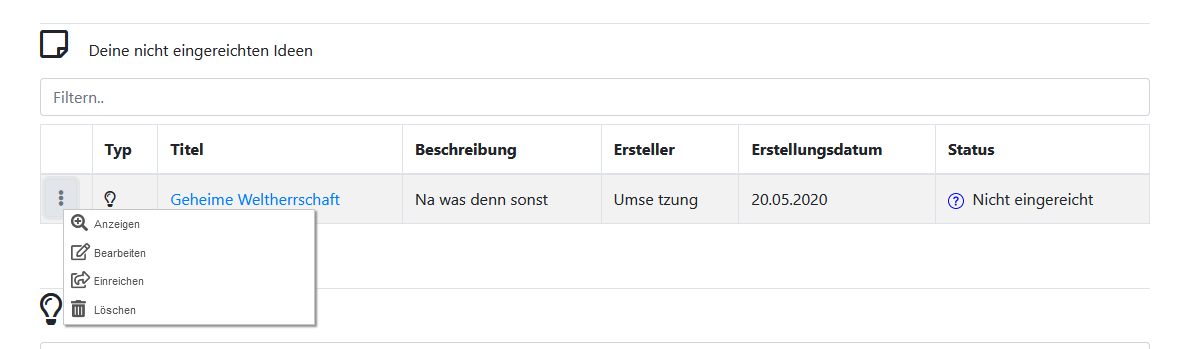
\includegraphics[width=1\textwidth]{img/rechtsklick-umsetzung.png}\\
        \source{Eigene Darstellung}
        \label{fig:rechtsklick}
    \end{minipage}
\end{figure}

\begin{figure}[hbt]
    \centering
    \begin{minipage}[t]{1\textwidth}
        \caption{Dropdown Umsetzung}
        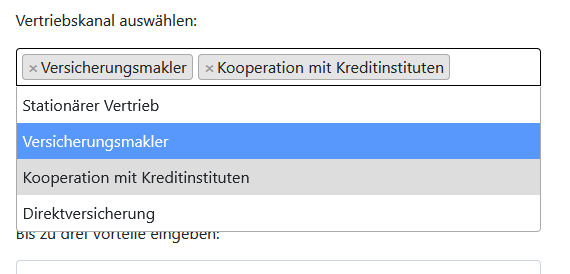
\includegraphics[width=0.5\textwidth]{img/dropdown-umsetzung.png}\\
        \source{Eigene Darstellung}
        \label{fig:dropdown}
    \end{minipage}
\end{figure}

Hervorzuheben ist, dass gegenüber des Konzeptes in der Umsetzung\footnote{Siehe Anhang \ref{GUI-Umsetzung} auf S.\pageref{GUI-Umsetzung}} einige Elemente hinzugekommen sind. Die wichtigsten hierbei sind das bereits genannte Rechtsklick Menü (Siehe \cref{fig:rechtsklick}). Sowie intelligente Dropdown Menüs (Siehe \cref{fig:dropdown}).
Diese sollen dem Nutzer die Möglichkeit geben intuitiv die Anwendung zu bedienen und erweitern diese durch dynamische Menüs welche sich in die Oberfläche einpassen.


    %!TEX root = ../Thesis.tex
\section{Konzepte}

\subsection{MVC-Pattern}
In unserer Anwendung benutzen wir das Architekturmuster Model View Controller.
Dieses Muster haben wir explizit ausgewählt, da Springboot zusammen mit Thymeleaf als Frontend hierfür sehr gut geeignet ist.


    %%%%%%%%%%%%%%%%%%%%%%%%%%%%%%%%

    %!TEX root = ../Thesis.tex
%! Author = JB
%! Date = 22.05.2020


\section{Projektplanung \textcolor{blue}{[Jonathan Brockhausen]}}

\subsection{Projektstrukturplan}
Das Projekt wurde von uns in vier Phasen aufgeteilt, \textit{Vorbereitung, Implementierung, Dokumentation \& Tests} und \textit{Abschluss.}
Der Projektstrukturplan ist im Anhang auf Seite \pageref{PSP} dargestellt.

\subsection{Soll-Ist-Vergleich}
Der vor dem Projekt von uns festgelegte und in der Präsentation des Fachkonzepts vermittelte Soll-Zustand ist die vollständige Umsetzung der Muss-Features und die in der angegebenen Reihenfolge begonnene Umsetzung der Kann-Features.
Im Anhang auf Seite \pageref{PM_SOLLIST} ist die Übersicht der Features dargestellt. Alle Soll-Features wurden anforderungsgemäß umgesetzt. Die Umsetzung der Kann-Features wurde gemäß der im Fachkonzept vorgestellten Priorisierung begonnen. Im Einklang mit dem gesamten Projekt wurde bei allen Features darauf geachtet, dass sie gut erweiter- und wartbar sind.\\
Die Programmierung einer REST-API wurde von uns als wichtigstes Kann-Feature priorisiert. Besonders im Unternehmenskontext kommen oft Schnittstellen zwischen sehr verschiedenen Programmen vor. Mit der Verwendung einer REST-API haben wir eine in gewissen Maßen standardisierte Schnittstelle, die durch das universelle Rückgabeformat JSON eine Anbindung im Unternehmen unterstützt. \\
Als zweites Kann-Feature haben wir ein Kontaktformular umgesetzt. Das Kontaktformular bietet für Benutzer und Administratoren gleichzeitig eine an das System angebundene Anlaufstelle für Problemmeldungen und Anfragen. Die Nachrichten laufen im Administrator-Interface auf und sind dort für alle Administratoren sicht- und bearbeitbar.\\
Der Administrator war das dritte Kann-Feature welches von Anfang an hoch priorisiert war und früh im Programm umgesetzt wurde. Neben der Benutzerverwaltung können Administratoren Spezialisten anlegen und weitere Einträge in den Vorlauftabellen anlegen. Außerdem kommen die oben genannten Kontaktnachrichten im Administrator-Interface an. Der modulare Aufbau des Administrator-Interfaces macht es einerseits übersichtlich für den Nutzer und andererseits gut erweiterbar um weitere Funktionen.\\
Die übrigen Kann-Features wurden zunächst nicht implementiert. Das Projekt kann jedoch um diese Features erweitert werden ohne bestehende Logik zu sehr verändern zu müssen. Eine Mail-Server-Anbindung wäre ein sinnvoller nächster Schritt der die Einbindung einiger weiterer Features und die Erweiterung von bestehenden Features ermöglicht (beispielsweise das Kontaktformular).

\subsection{Arbeitsaufteilung}
\label{Arbeitsaufteilung}

Für die Arbeitsaufteilung wurden die regelmäßigen Synchronisations-Calls genutzt. Die anstehenden Aufgaben wurden in Arbeitspakete aufgeteilt und gemeinsam im Team verteilt. Hierbei wurden persönliche Fähigkeiten und Vertrautheit mit der speziellen Code-Stelle besonders in Betracht gezogen. Aufgrund der oben erwähnten All-Hands-On-Deck-Methode wurde sichergestellt, dass alle Teammitglieder informiert waren, wer an welcher Stelle arbeitet und somit Konflikte im Code vermieden.
Für das Festhalten der Arbeitspakete und der individuellen Fortschritte wurde das Projektmanagement-Tool OpenProject verwendet. Der Umfang des Projekts lässt über die Sinnhaftigkeit eines dedizierten Projektmanagementtools sicherlich streiten, aber unter dem Strich konnte so deutlich besser eine Struktur in die Arbeitsaufteilung gebracht werden. \\

    %!TEX root = ../Thesis.tex
%! Author = PR
%! Date = 27.05.2020


\section{Schlussbetrachtung \textcolor{blue}{[Philipp Röring]}}

\subsection{Bewertung}
In Anhang~\ref{PM_SOLLIST} ist zu sehen, dass alle Muss-Features der Anwendung implementiert wurden. Die Kann-Features wurden gemäß der
vorgestellten Priorisierung implementiert. Es gab somit bezüglich der Implementierung keine Abweichungen von der Projektplanung.
\\
Trotz der Aufteilung des Entwicklungsaufwandes wurde bei Unklarheiten mehrmals zusammen nach Lösungen gesucht. Auch im Rahmen der
Qualitätssicherung wurde der Quelltext gemeinsam überprüft und besprochen. Unabhängig davon stand es jedem Entwickler frei, nach Absprache den Quelltext eines anderen zu
überarbeiten, wenn er Fehler bzw. Unschönheiten in diesem gefunden hat. Die Zusammenarbeit wurde allgemein als sehr gut eingeschätzt. Lediglich die rein digitale Kommunikation
aufgrund der aktuellen Covid-19 Situation hat die Zusammenarbeit in geringem Maße erschwert. Die Entwickler sind sich jedoch einig, dass dies nicht die hohe Qualität
der erstellten Anwendung gesenkt hat.
\\
Durch den sehr frühen Beginn der Entwicklung konnten die Laufzeit des Gesamtprojektes sowie die einzeln vergebenen Deadlines
für die Entwickler eingehalten werden. Auch das Aneignen von Know-How über Spring, Spring-boot und Thymeleaf konnte
in die Projektlaufzeit integriert werden.
\\
In den letzten Releases der Anwendung liefen alle Tests, die automatischen sowie die manuellen GUI-Tests, fehlerfrei durch. Es folgt eine kurze
eigene Bewertung der Qualität der Anwendung (1-10 Punkte).

\begin{longtable}{|p{0.14\textwidth}|p{0.15\textwidth}|p{0.09\textwidth}|p{0.15\textwidth}|p{0.17\textwidth}|p{0.15\textwidth}|}
    \caption{Bewertung der Anwendung}\\
    \hline
    Änderbarkeit & Benutzbarkeit & Effizienz & Funktionalität & Übertragbarkeit & Zuverlässigkeit\\
    \hline
    8 & 8 & 6 & 8 & 10 & 9 \\
    \hline
\end{longtable}

Die etwas niedrige Effizienz im Gegensatz zu sehr hoher Übertragbarkeit ist auf die Java-Programmiersprache zurückzuführen.
Darüber hinaus wurde zwar während der Entwicklung auf Performanz geachtet, allerdings wurde diese aufgrund
der mittleren Benutzeranzahl nicht gegenüber anderen Qualitätsmerkmalen priorisiert.
Die Bewertung der Zuverlässigkeit wurde nach dem ständigen Bestehen der Tests sowie dem fehlenden Aufkommen von Programmabbrüchen bewertet.
Die hohe Änderbarkeit resultiert aus strukturiertem Quelltext, bei dem sich an die Standard-Struktur von Spring Projekten gehalten wurde.
Die Funktionalität und Benutzbarkeit wurde von Dritt-Testern bewertet.

\subsection{Fazit}
Der Soll-Ist Vergleich hat gezeigt, dass das Entwicklerteam gut zusammenarbeiten kann und für weitere Projekte bestens geeignet ist.
Es wäre allerdings von Vorteil, wenn die Entwickler für weitere Projekte eine Vorlaufzeit bekommen um sich in benötigte
Technologien einzuarbeiten. Darüber hinaus ist davon auszugehen, dass eine persönliche Kommunikation die Synergie des Teams
verstärken würde.










%%%%%%%%%%%%%%%%%%%%%%%%%%%%%%%%%%%%%%%%%%%%%%%%%%%%%%%%%%%%%%%%%%%%%%%
%% Anhang
%%%%%%%%%%%%%%%%%%%%%%%%%%%%%%%%%%%%%%%%%%%%%%%%%%%%%%%%%%%%%%%%%%%%%%%

    %!TEX root = ../Thesis.tex

\section*{Anhang}
\addcontentsline{toc}{section}{Anhang}
\fancyhead[R]{Anhang}

\anhangsverzeichnis

\anhang{Testdurchführung \textcolor{blue}{[Julius Figge]}}

\begin{center}
    \label{fig:testdurchf}
    \begin{longtable}{|p{0.4\textwidth}|p{0.3\textwidth}|p{0.2\textwidth}|}
        \caption{GUI-Testdurchführung}\\
        \hline
        Aktion & erwartetes Ergebnis & Reaktion\\
        \hline
        \hline

        \textbf{Registrieren eines neuen Nutzers} & &\\
        \hline
        Bereits bestehenden Nutzernamen verwenden (admin) & Fehlermeldung - Nutzername existiert bereits &\\
        \hline
        zu kurzer Nutzername (<3) & Fehlermeldung - Daten falsch &\\
        \hline
        zu kurzes Passwort (<=7) & Fehlermeldung - zu kurzes Passwort &\\
        \hline
        nicht übereinstimmende Passwörter & Fehlermeldung - nicht stimmende Passwort &\\
        \hline
        mit korrekten Daten & eingeloggt sein &\\
        \hline
        \hline

        \textbf{Ausloggen aus dem Account} & ausgeloggt sein &\\
        \hline
        \hline

        \textbf{Einloggen in erstellten Account} & &\\
        \hline
        mit falschem Passwort & Fehlermeldung &\\
        \hline
        mit falschem Nutzernamen & Fehlermeldung &\\
        \hline
        mit richtigem Passwort & eingeloggt sein &\\
        \hline
        \hline

        \textbf{Erstellen von beispielhaften Ideen} & &\\
        \hline
        Erstellen einer \enquote{internen Idee} & Idee erscheint in Tabelle nicht eingereichter Ideen &\\
        \hline
        Erstellen einer \enquote{Produkt-Idee} & Idee erscheint in Tabelle nicht eingereichter Ideen &\\
        \hline
        Erstellen einer beliebigen Idee mit fehlerhaften Werten & Fehlerhafte Attribute werden hervorgehoben &\\
        \hline
        Erstellen einer Idee von der bereits selber Name bei selbem Typ vorhanden & Fehlermeldung über Duplikat &\\
        \hline
        Bearbeiten der internen Idee & Änderungen werden übernommen &\\
        \hline
        Bearbeiten der Produkt-Idee & Änderungen werden übernommen &\\
        \hline
        \hline

        \textbf{Ideenübersicht} & &\\
        \hline
        Filtern der nicht eingereichten Ideen nach Attributen & nur Ideen mit passenden Attributen werden angezeigt &\\
        \hline
        Einreichen der erstellten Ideen & erfolgreicher Transfer in jeweilige Tabelle &\\
        \hline
        \hline

        \textbf{Ausloggen aus dem Account} & ausgeloggt sein &\\
        \hline
        \hline

        \textbf{Idee Übersicht als nicht eingeloggter Nutzer} & &\\
        \hline
        Filtern der Ideen in beiden Tabellen & nur Ideen mit passenden Attributen werden angezeigt &\\
        \hline
        \hline

        \textbf{Kontaktformular} & & \\
        \hline
        Kontaktformular im Footer aufrufen & Kontaktformular erscheint & \\
        \hline
        Nachricht mit Titel, Nachricht und eigener E-Mail-Adresse absenden & Nachricht abgesendet & \\
        \hline
        Nachricht mit Titel, Nachricht und falsch formatierter E-Mail-Adresse absenden & Fehler & \\
        \hline
        \hline

        \textbf{Spezialist für \enquote{internen Idee}} & &\\
        \hline
        Einloggen als passender (Ideen sollten ihm zugewiesen sein) Spezialist (Zugangsdaten siehe \texttt{Manual.md})& eingeloggt sein &\\
        \hline
        Übersicht zu entscheidender Ideen filtern & nur Ideen mit passenden Attributen werden angezeigt &\\
        \hline
        Entscheiden ohne Begründung & fehlendes Attribut wird hervorgehoben &\\
        \hline
        Idee in Ideenspeicher verschieben & Idee liegt in Ideenspeicher &\\
        \hline
        \hline

        \textbf{Spezialist für \enquote{Produkt-Idee}} & &\\
        \hline
        Account zu anderem Spezialist wechseln & Eingeloggt und Idee liegt in Ideenspeicher &\\
        \hline
        Entscheiden über Idee aus Ideenspeicher mit Auswahl  \enquote{zur Entscheidung freigegeben} & Idee liegt in eigenen zu entscheidenden Ideen &\\
        \hline
        Idee aus Entscheidungsübersicht bewerten & Idee erscheint auf passender Tabelle in Ideenübersicht &\\
        \hline
        Ausloggen & Ausgeloggt und angenommene Idee mit Begründung in Ideenübersicht &\\
        \hline
        \hline

        \textbf{Administrator} & &\\
        \hline
        Account zu Administrator wechseln (Zugangsdaten siehe \texttt{Manual.md})& Eingeloggt auf Admin-Seite &\\
        \hline
        Existierende User anschauen & registrierter Account sowie alle Spezialisten werden aufgelistet &\\
        \hline
        Neuen Fachspezialisten anlegen & Spezialist taucht in Userliste auf &\\
        \hline
        Neue Produktsparte anlegen & Produktsparte angelegt &\\
        \hline
        Neue Handlungsfeld anlegen & Handlungsfeld angelegt &\\
        \hline
        Neue Zielgruppe anlegen & Zielgruppe angelegt &\\
        \hline
        Neue Vertriebskanal anlegen & Vertriebskanal angelegt &\\
        \hline
        Vertriebskanal mit dem selben Titel anlegen & Fehler wird angezeigt &\\
        \hline
        Kontaktnachricht ansehen und als beantwortet kennzeichnen & Keine ungelesenen Nachrichten &\\
        \hline
        Ausloggen & Ausgeloggt &\\
        \hline
    \end{longtable}
\end{center}

\clearpage
\pagebreak

\anhang{Weitere Use-Cases \textcolor{blue}{[Julius Figge]}}\label{Anhang-Use-Cases}

\subanhang{Administrator}\label{Anhang-Admin}
\begin{figure}[h]
    \centering
    \begin{minipage}[t]{1\textwidth}
        \caption{Administrator - Use-Case Diagramm}
        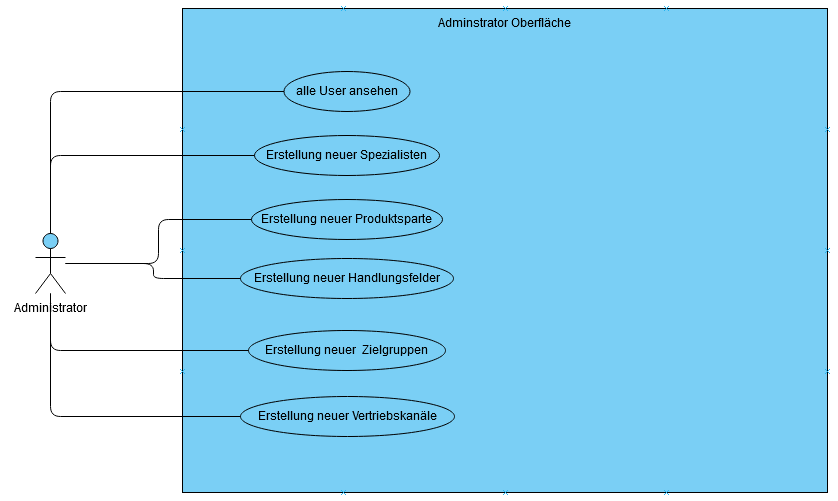
\includegraphics[width=1\textwidth]{img/admin-use-case.png}\\
        \source{Eigene Darstellung}
    \end{minipage}
\end{figure}

\subanhang{Kontaktformular}\label{Anhang-Kontakt}
\begin{figure}[h]
    \centering
    \begin{minipage}[t]{1\textwidth}
        \caption{Kontaktformular - Use-Case Diagramm}
        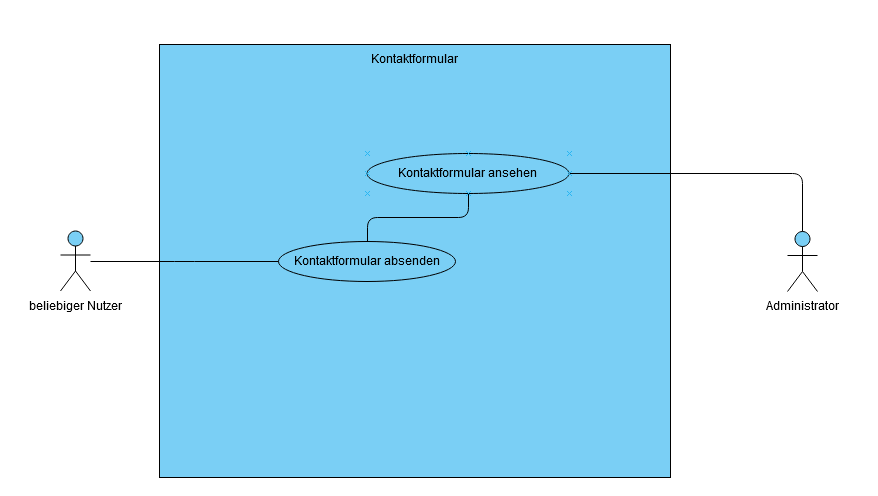
\includegraphics[width=1\textwidth]{img/kontakt-use-case.png}\\
        \source{Eigene Darstellung}
    \end{minipage}
\end{figure}

\clearpage
\pagebreak

\anhang{GUI-Konzept \textcolor{blue}{[Julius Figge]}}
\label{GUI-Konzept}
\subanhang{Konzept}

\begin{figure}[hbt]
    \centering
    \begin{minipage}[t]{1\textwidth}
        \caption{GUI-Konzept - Login}
        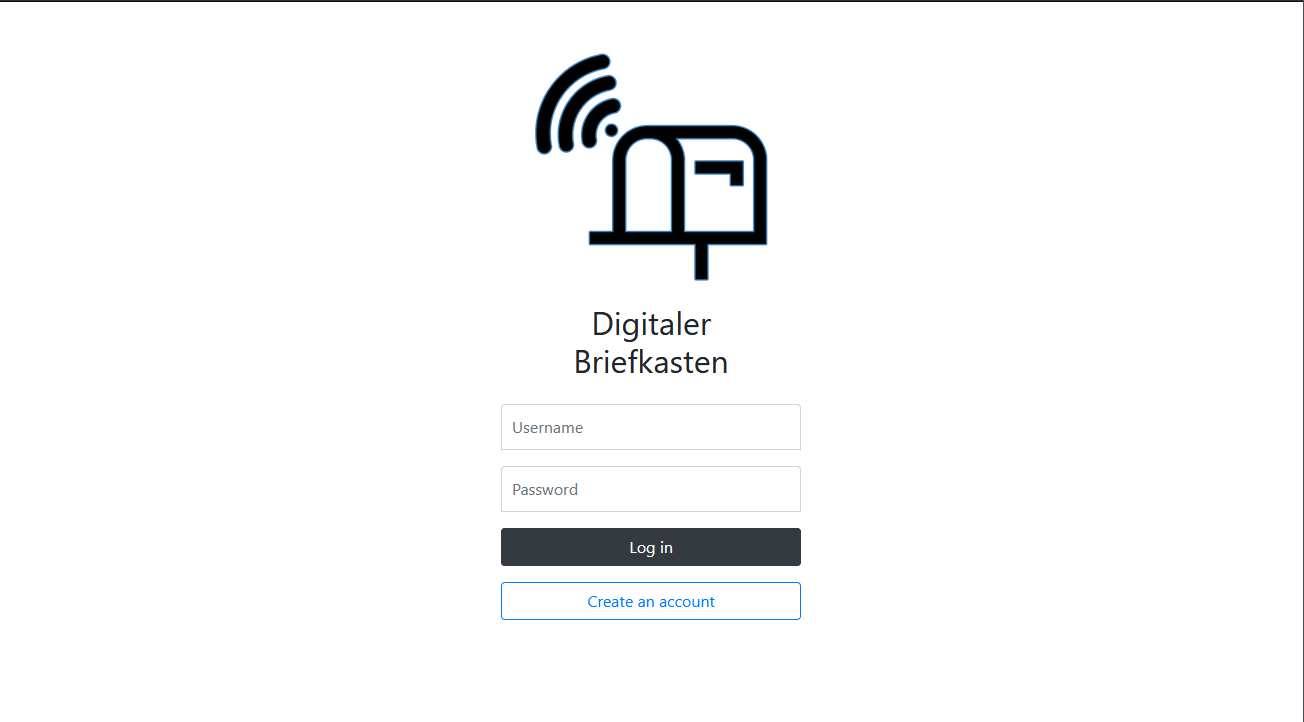
\includegraphics[width=1\textwidth]{img/login-konzept.png}\\
        \source{Eigene Darstellung}
        \label{fig:login}
    \end{minipage}
\end{figure}

\begin{figure}[h]
    \centering
    \begin{minipage}[t]{1\textwidth}
        \caption{GUI-Konzept - Registrierung }
        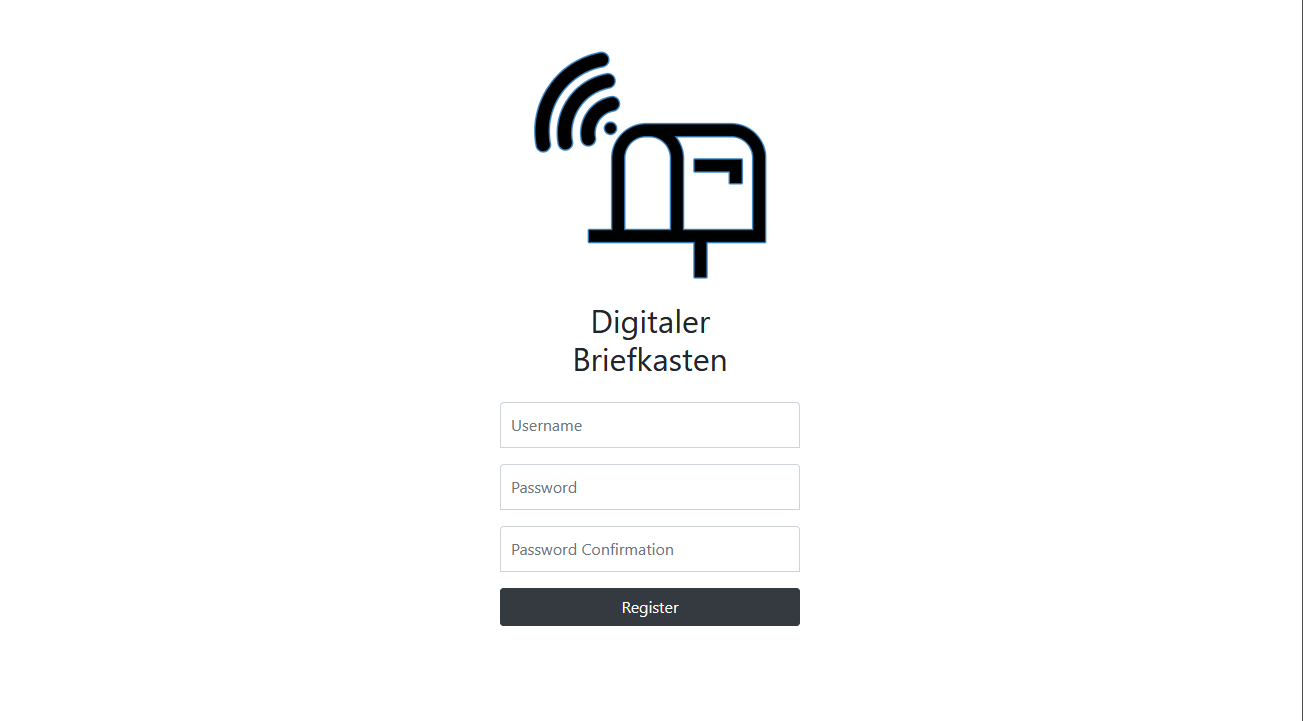
\includegraphics[width=1\textwidth]{img/registrierung-konzept.png}\\
        \source{Eigene Darstellung}
    \end{minipage}
\end{figure}

\begin{figure}[h]
    \centering
    \begin{minipage}[t]{1\textwidth}
        \caption{GUI-Konzept - Willkommen}
        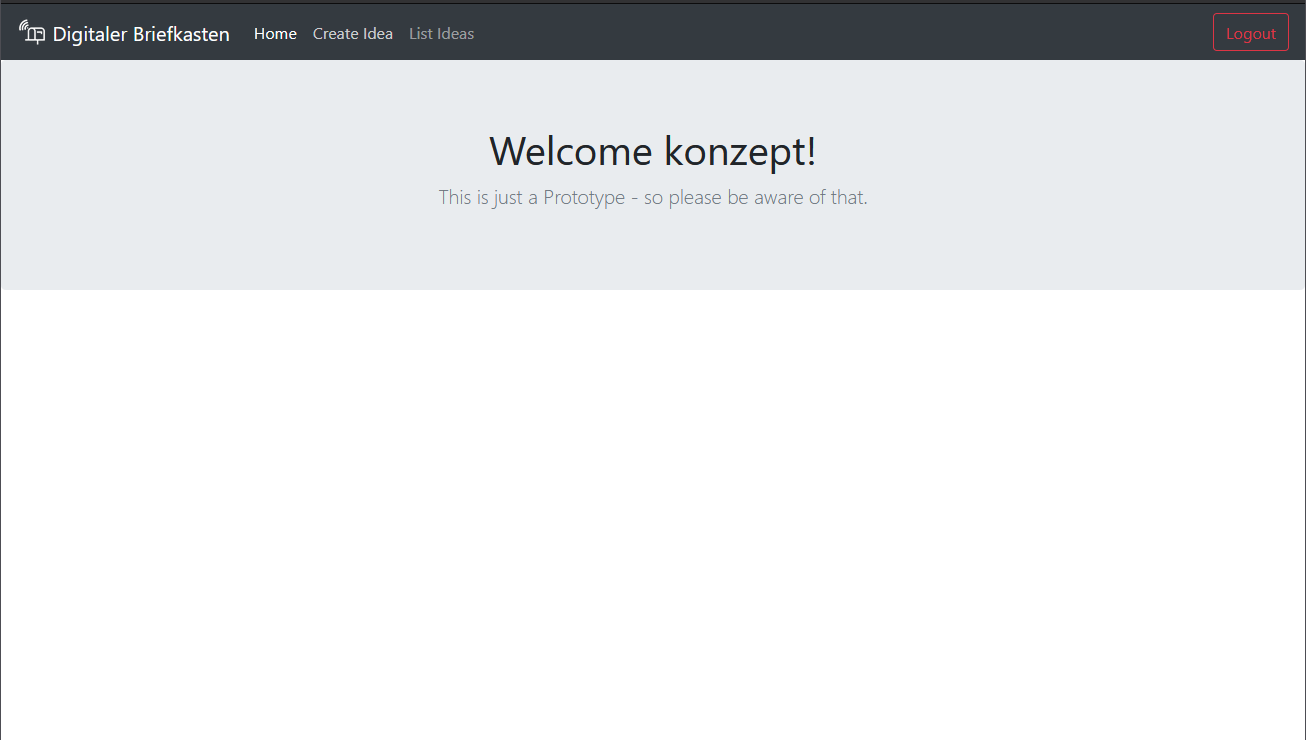
\includegraphics[width=1\textwidth]{img/welcome-konzept.png}\\
        \source{Eigene Darstellung}
    \end{minipage}
\end{figure}

\begin{figure}[h]
    \centering
    \begin{minipage}[t]{1\textwidth}
        \caption{GUI-Konzept - Idee erstellen}
        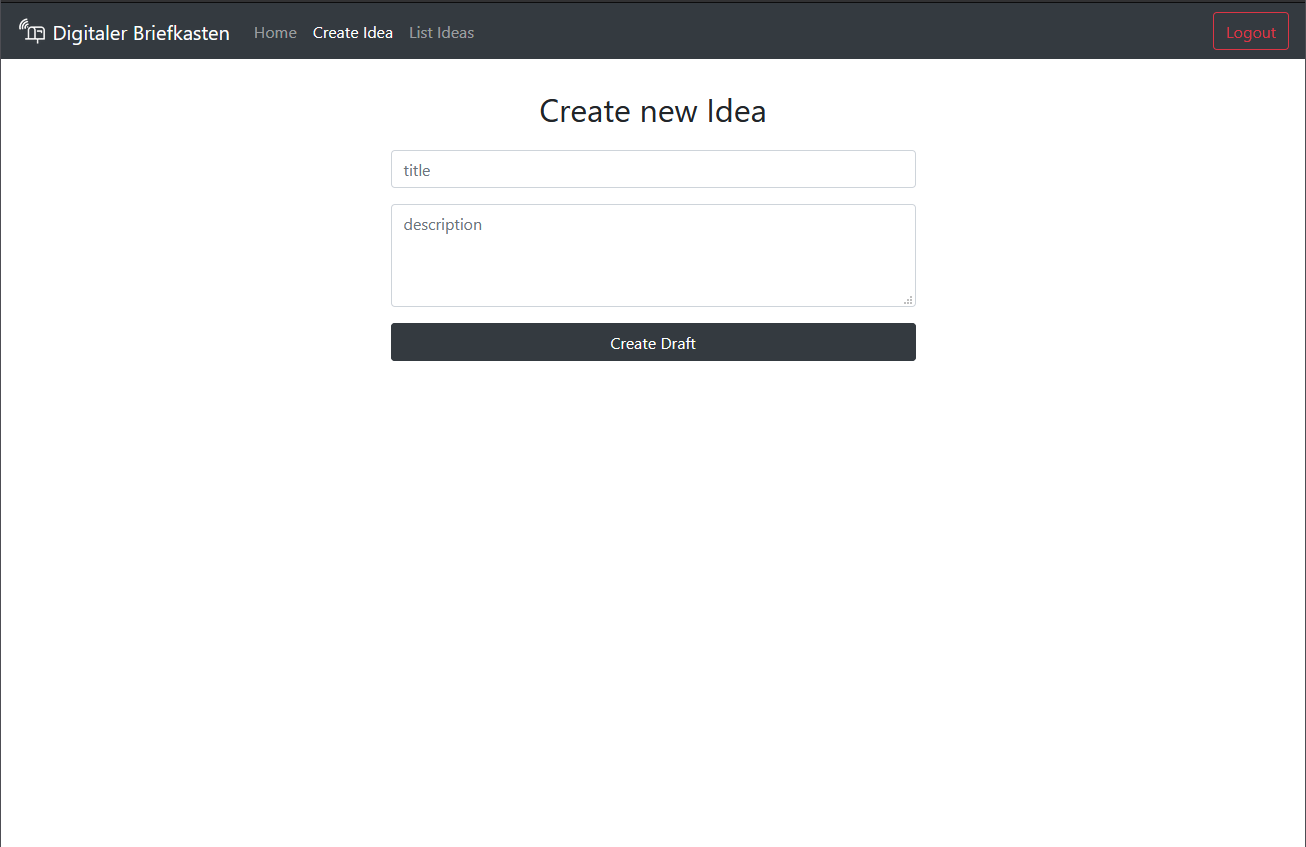
\includegraphics[width=1\textwidth]{img/createIdea-konzept.png}\\
        \source{Eigene Darstellung}
    \end{minipage}
\end{figure}

\clearpage
\pagebreak

\subanhang{Umsetzung}\label{GUI-Umsetzung}

Die im folgenden dargestellten GUI Bestandteile stellen die wichtigsten Teile der Oberfläche dar. Auf die Abbildung aller Bestandteile wurde aufgrund der zu großen Menge, zur Wahrung der Übersichtlichkeit, verzichtet.

\begin{figure}[h]
    \centering
    \begin{minipage}[t]{1\textwidth}
        \caption{GUI-Umsetzung - Login }
        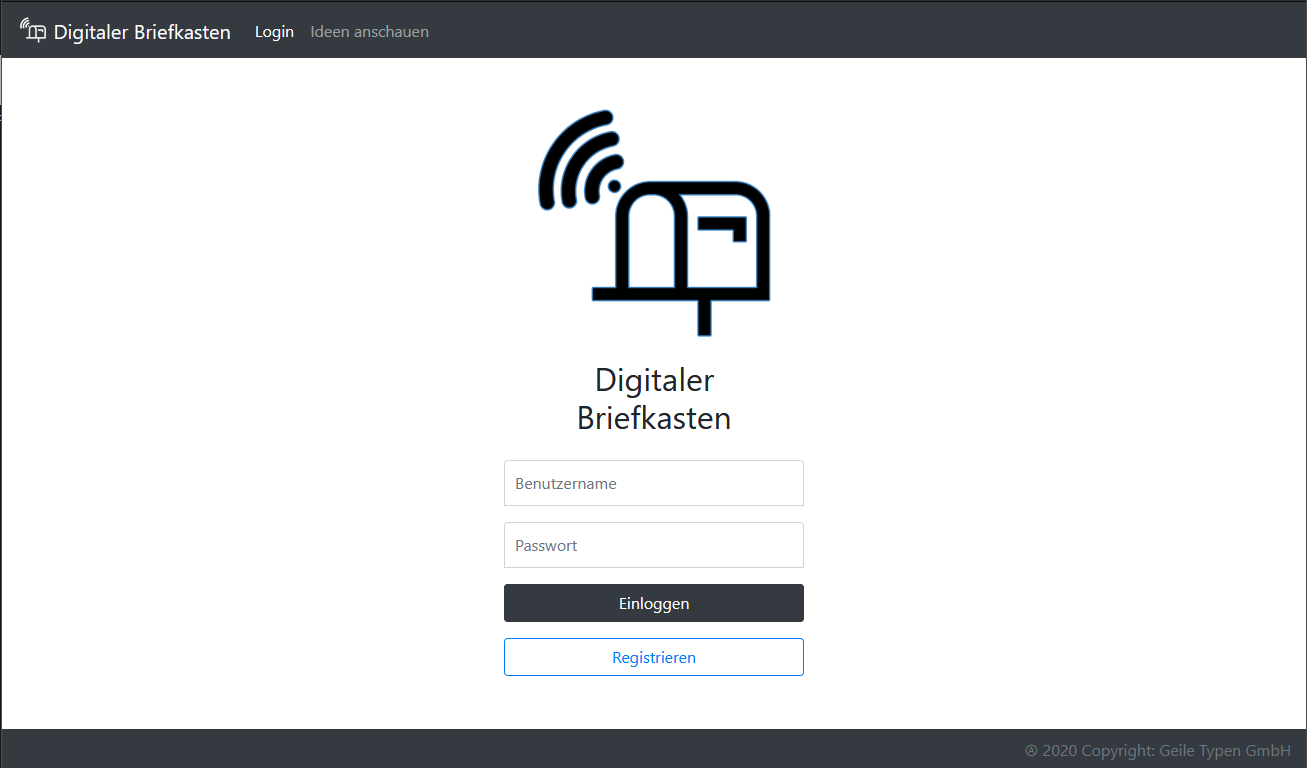
\includegraphics[width=1\textwidth]{img/login-umsetzung.png}\\
        \source{Eigene Darstellung}
    \end{minipage}
\end{figure}

\begin{figure}[h]
    \centering
    \begin{minipage}[t]{1\textwidth}
        \caption{GUI-Umsetzung - Registrierung }
        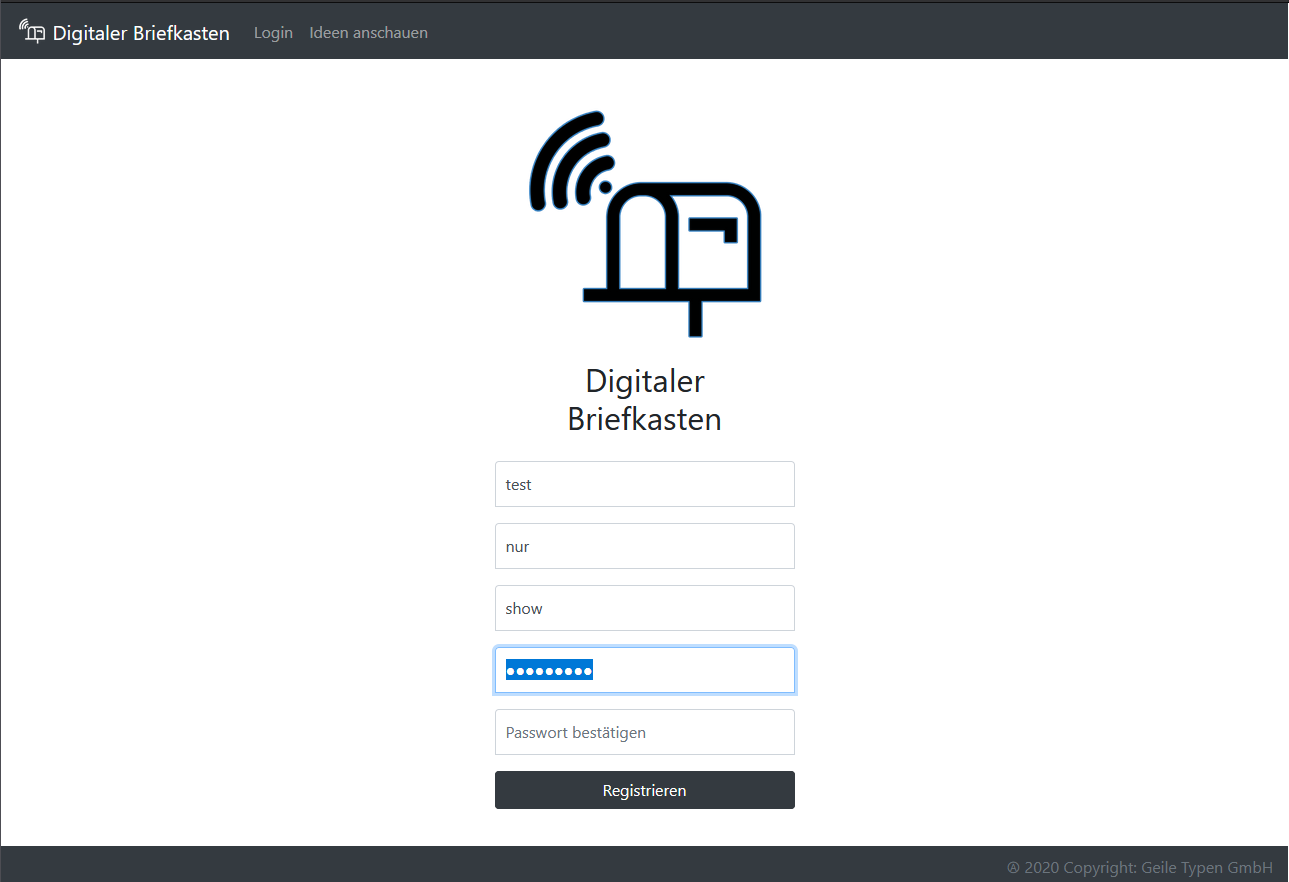
\includegraphics[width=1\textwidth]{img/registrierung-umsetzung.png}\\
        \source{Eigene Darstellung}
    \end{minipage}
\end{figure}

\begin{figure}[h]
    \centering
    \begin{minipage}[t]{1\textwidth}
        \caption{GUI-Umsetzung - Ideen}
        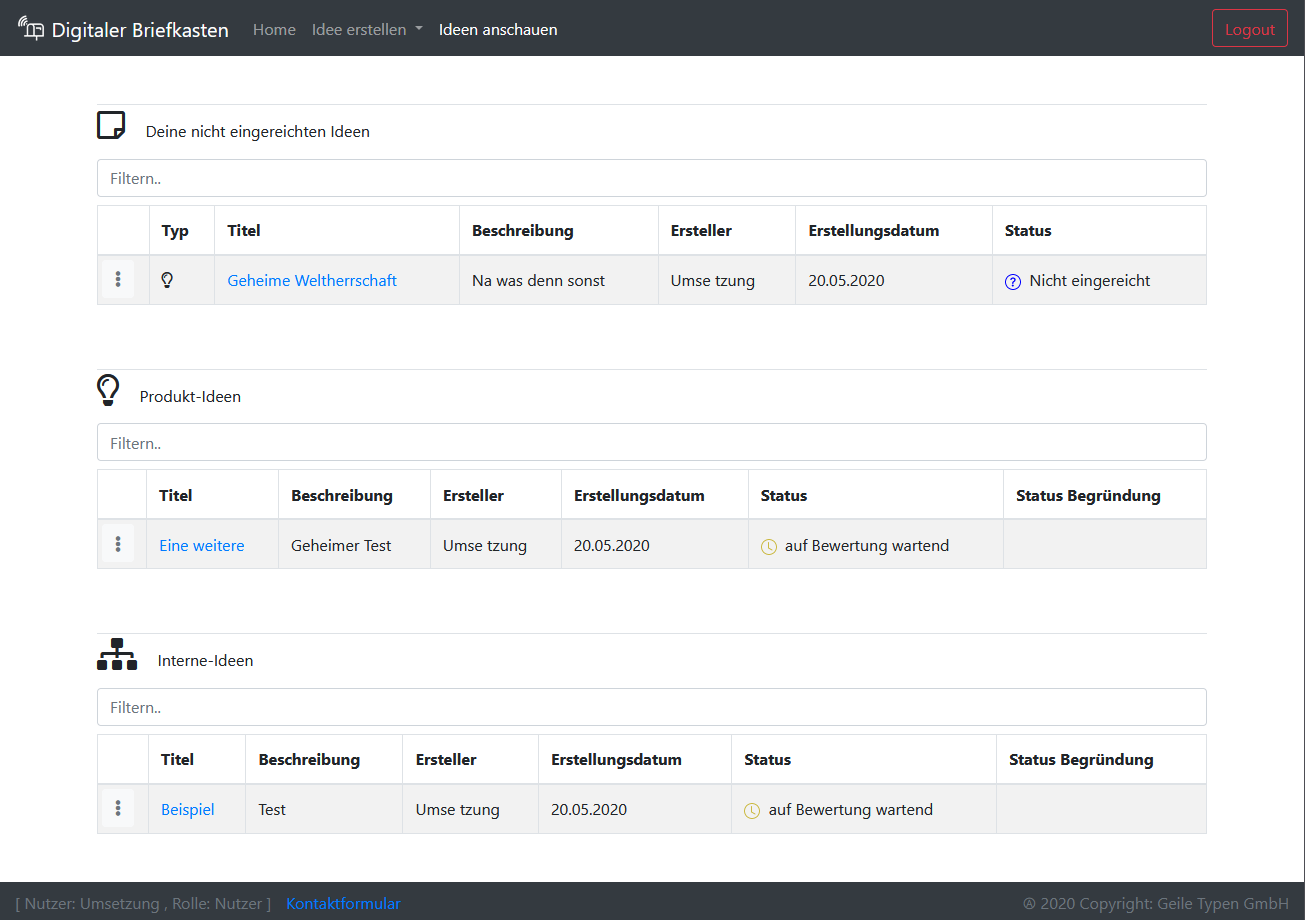
\includegraphics[width=1\textwidth]{img/ideen-umsetzung.png}\\
        \source{Eigene Darstellung}
    \end{minipage}
\end{figure}

\begin{figure}[h]
    \centering
    \begin{minipage}[t]{1\textwidth}
        \caption{GUI-Umsetzung - Idee erstellen }
        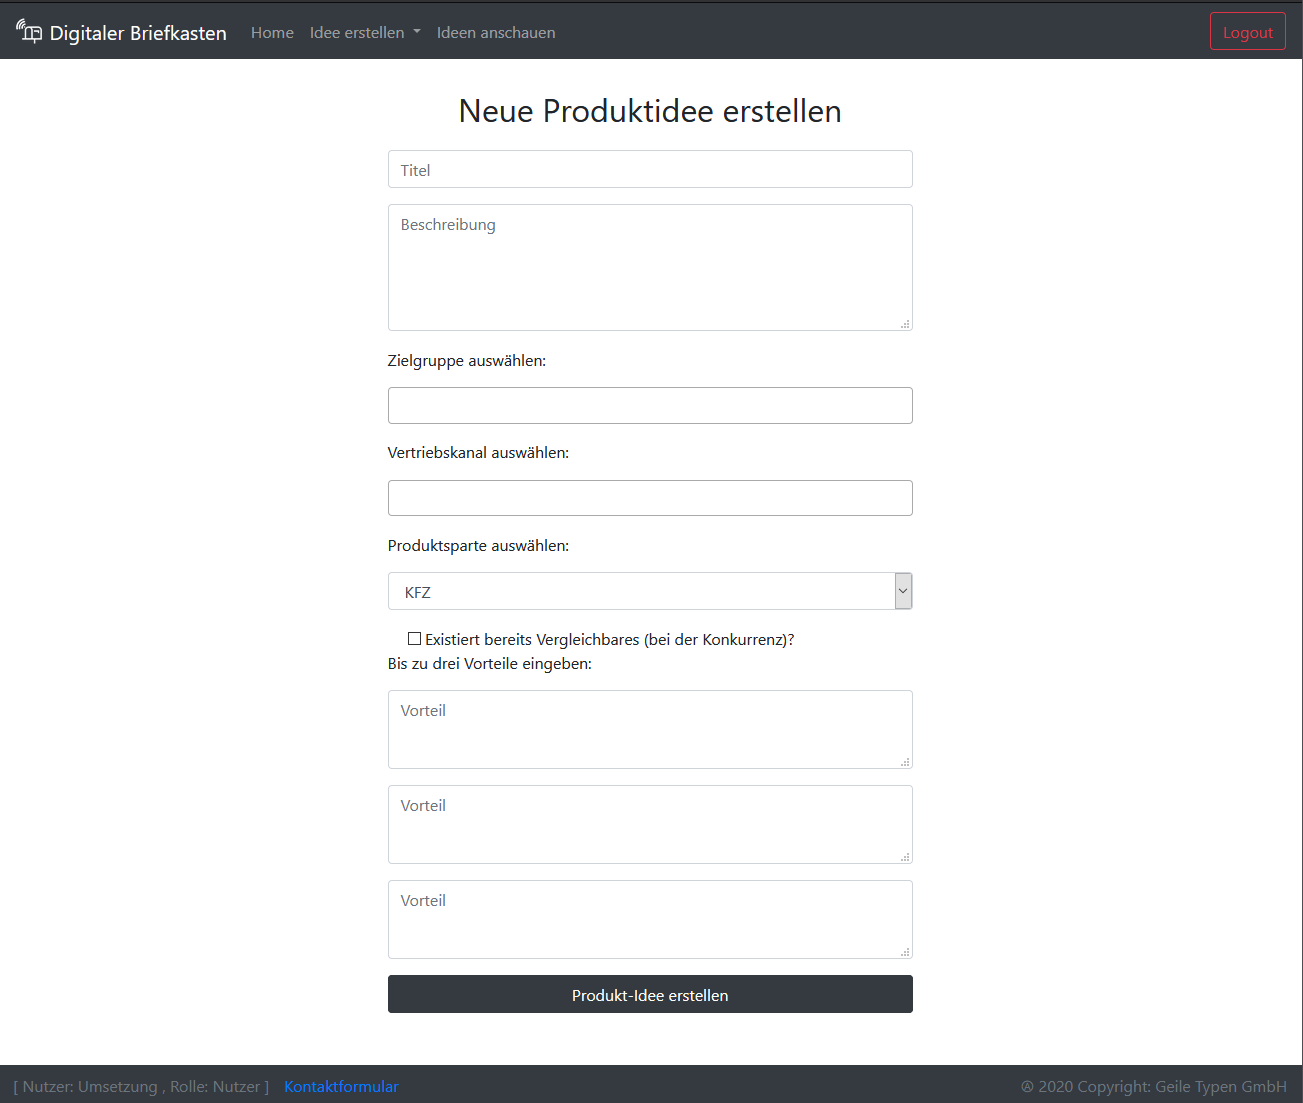
\includegraphics[width=1\textwidth]{img/createIdea-umsetzung.png}\\
        \source{Eigene Darstellung}
    \end{minipage}
\end{figure}

\begin{figure}[h]
    \centering
    \begin{minipage}[t]{1\textwidth}
        \caption{GUI-Umsetzung - Idee ansehen }
        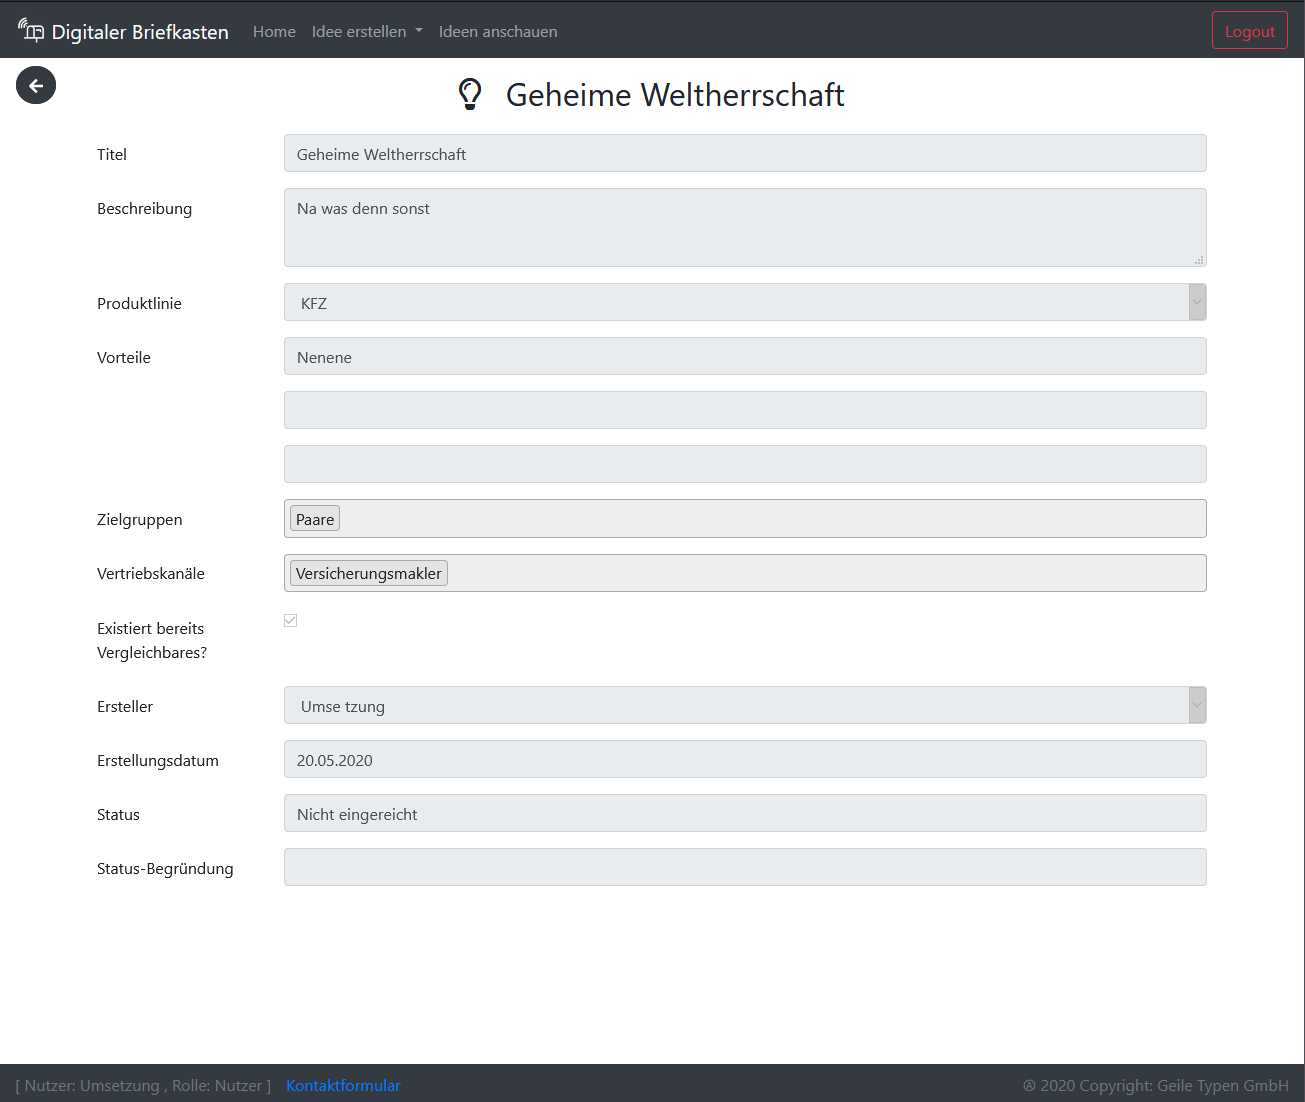
\includegraphics[width=1\textwidth]{img/idee-umsetzung.png}\\
        \source{Eigene Darstellung}
    \end{minipage}
\end{figure}

\begin{figure}[h]
    \centering
    \begin{minipage}[t]{1\textwidth}
        \caption{GUI-Umsetzung - Admin Ansicht }
        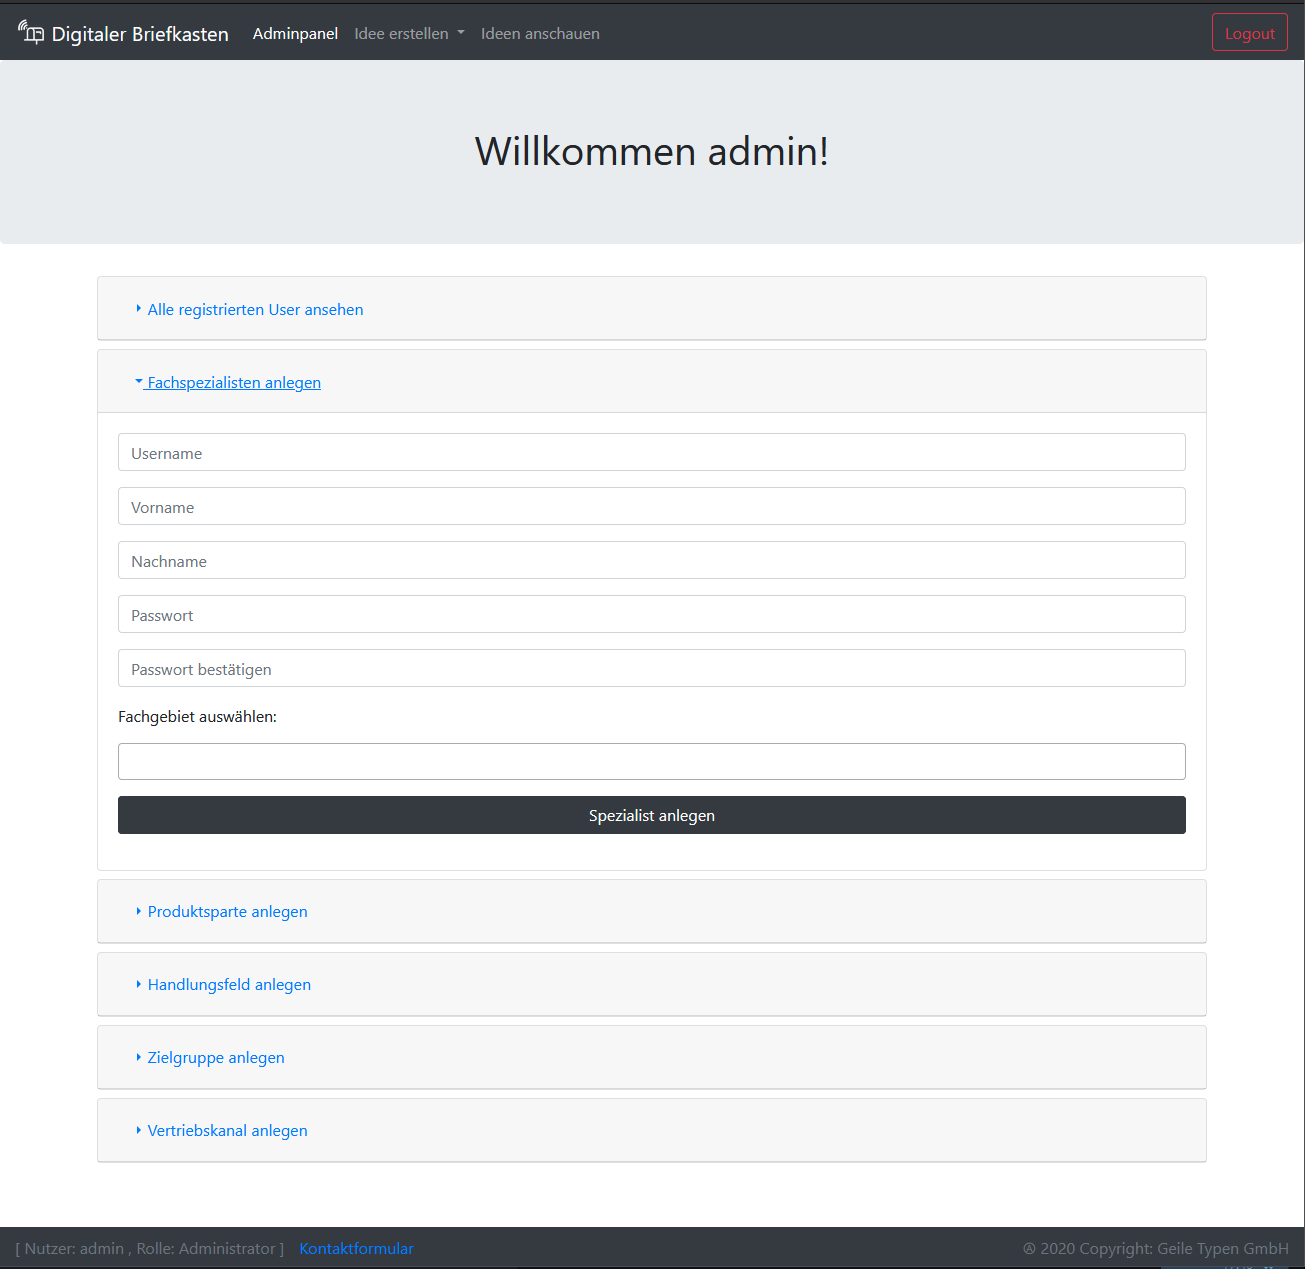
\includegraphics[width=1\textwidth]{img/admin-umsetzung.png}\\
        \source{Eigene Darstellung}
    \end{minipage}
\end{figure}

\begin{figure}[h]
    \centering
    \begin{minipage}[t]{1\textwidth}
        \caption{GUI-Umsetzung - Spezialist Ansicht }
        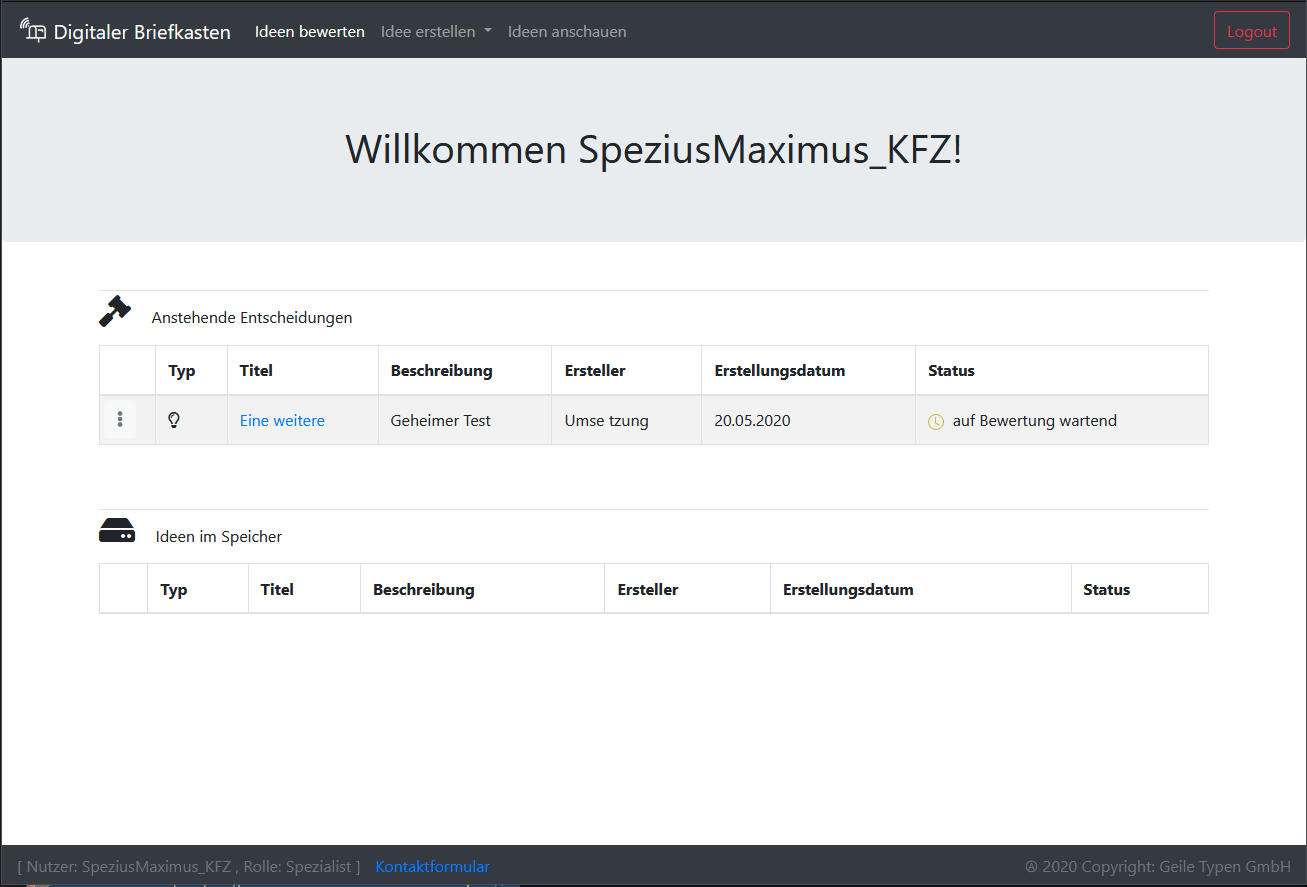
\includegraphics[width=1\textwidth]{img/spezialist-umsetzung.png}\\
        \source{Eigene Darstellung}
    \end{minipage}
\end{figure}

\pagebreak
\clearpage

\anhang{Projektplanung}
\subanhang{Projektstrukturplan}
\label{PSP}
\begin{figure}[h]
    \centering
    \begin{minipage}[t]{1\textwidth}
        \caption{Projektstrukturplan}
        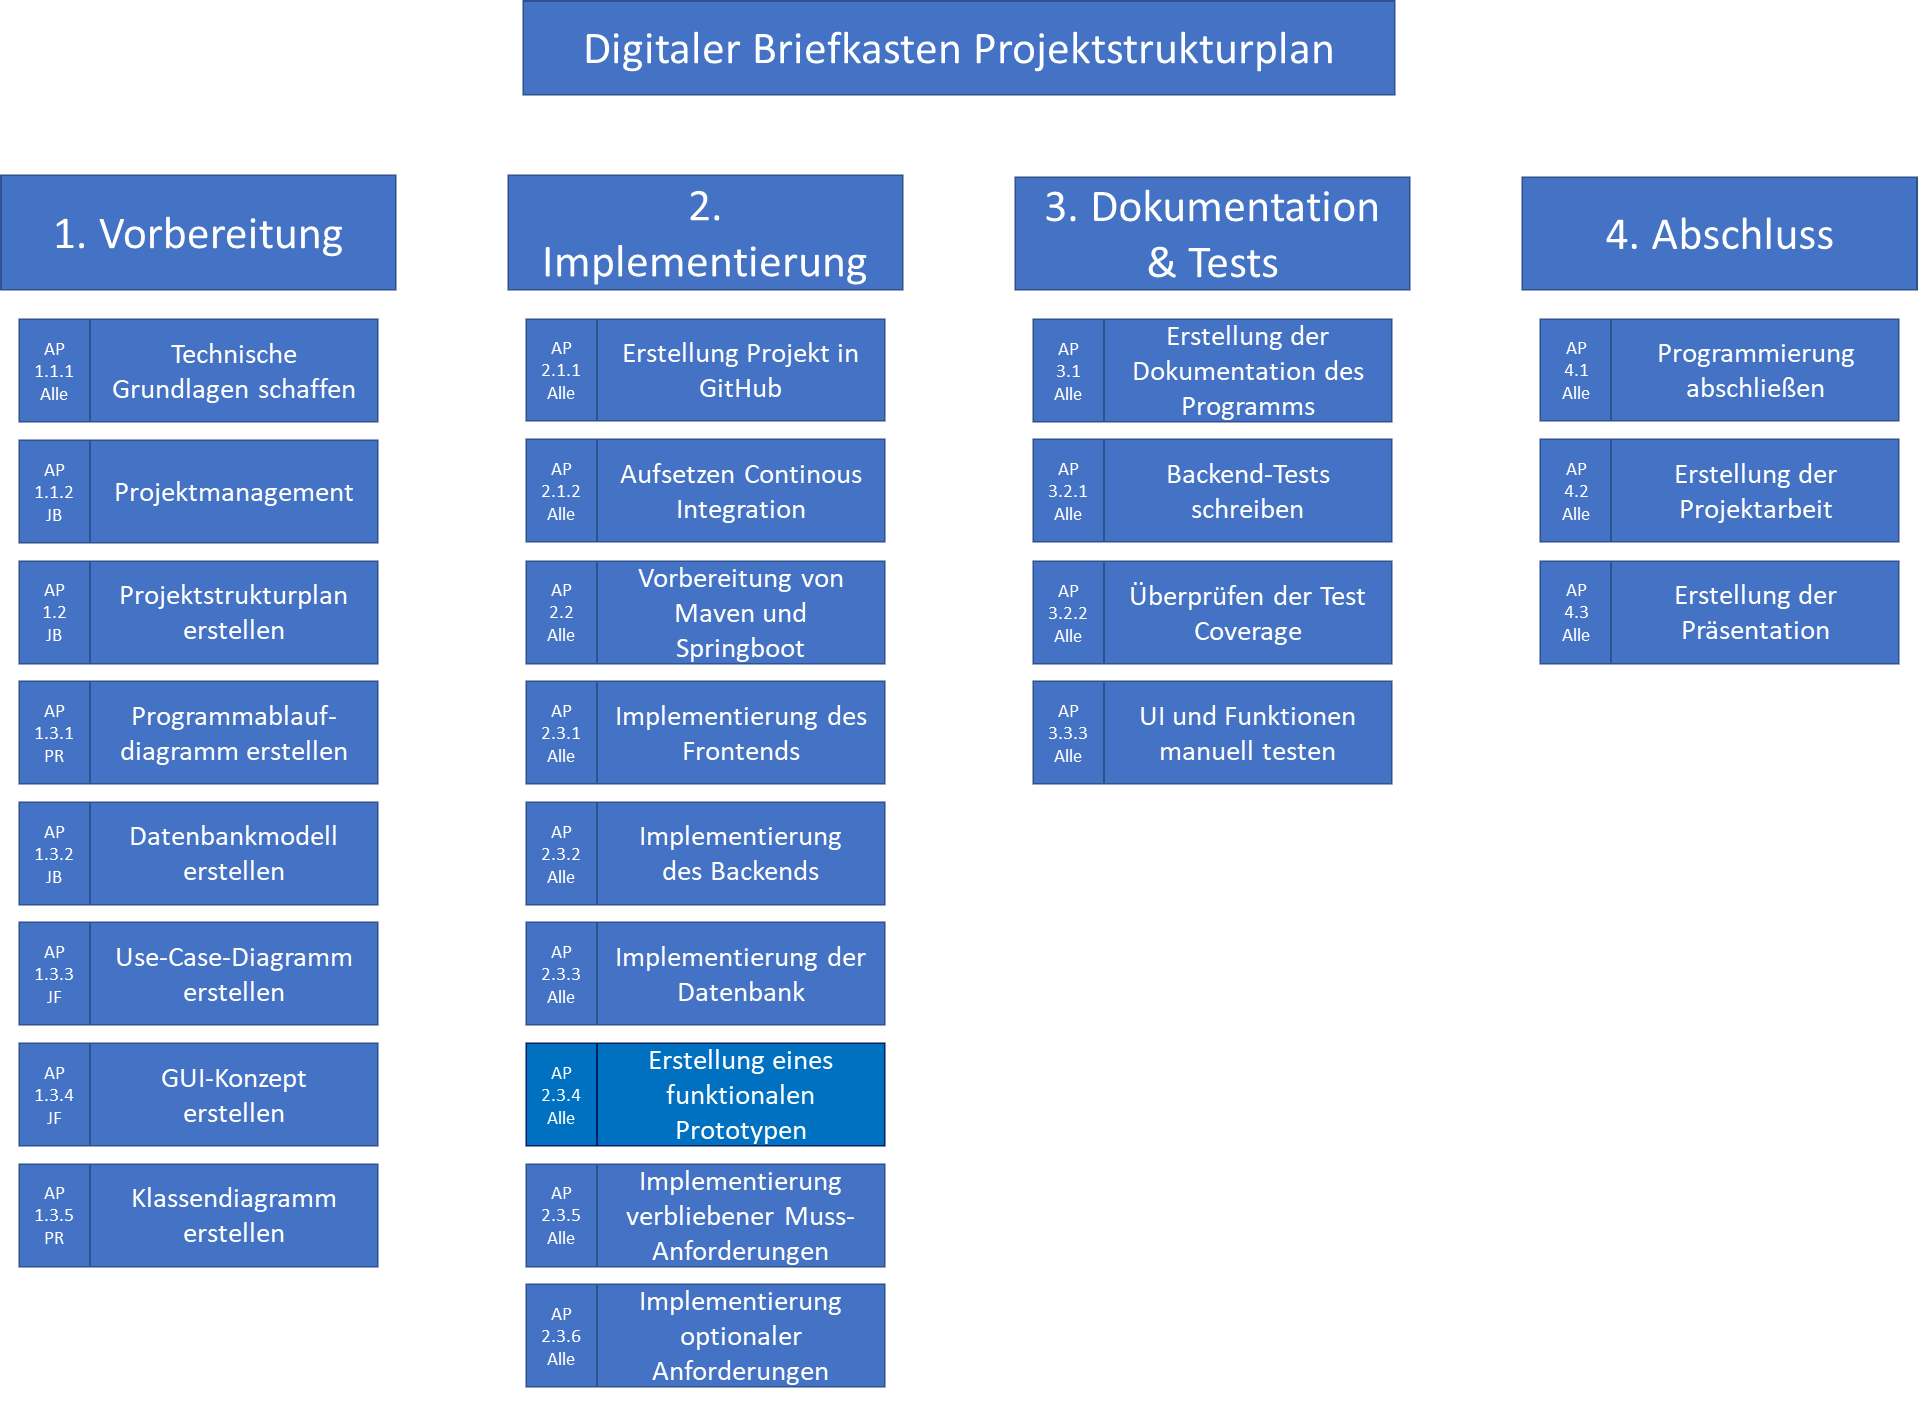
\includegraphics[width=1\textwidth]{img/PSP.png}\\
        \source{Eigene Darstellung}
    \end{minipage}
\end{figure}

\pagebreak
\clearpage

\subanhang{Soll-Ist-Vergleich Muss- und Kann-Features}
\label{PM_SOLLIST}
\begin{center}
    \begin{tabularx}{\linewidth}{
        |p{\dimexpr.09\linewidth-2\tabcolsep-1.3333\arrayrulewidth}% column 2
        |p{\dimexpr.66\linewidth-2\tabcolsep-1.3333\arrayrulewidth}% column 1
        |p{\dimexpr.25\linewidth-2\tabcolsep-1.3333\arrayrulewidth}|% column 3
    }
        \hline
        & Anforderung & Umsetzung \\ \hline
        Muss & Noch nicht registrierte Mitarbeiter können sich am System registrieren & Umgesetzt \\ \hline
        Muss & Registrierte Mitarbeiter können sich am System anmelden & Umgesetzt \\ \hline
        Muss & Registrierte Mitarbeiter können neue Ideen erfassen & Umgesetzt \\ \hline
        Muss & Registrierte Mitarbeiter können sich eine Liste ihrer eingereichten Ideen anzeigen lassen & Umgesetzt \\ \hline
        Muss & Registrierte Mitarbeiter können ihre Ideen solange bearbeiten oder auch löschen solange dieses noch nicht zur Bewertung an einen Fachspezialisten übergeben wurden. & Umgesetzt \\ \hline
        Muss & Nicht registrierte Mitarbeiter können vorhandene Ideen lesen, sich eine Übersicht der Ideen anzeigen lassen und die Übersicht filtern & Umgesetzt \\ \hline
        Muss & Diese Funktionen stehen auch registrierten Mitarbeitern zur Verfügung & Umgesetzt \\ \hline
        Muss & Neue Ideen werden Fachspezialisten zur Bewertung zugeordnet & Umgesetzt \\ \hline
        Muss & Die Zuordnung erfolgt automatisch sobald die Idee vom registrierten Mitarbeiter zur Bewertung eingereicht wurde & Umgesetzt \\ \hline
        Muss & Fachspezialisten können eine Idee entweder annehmen, ablehnen oder für einen späteren Zeitpunkt in einen sog. Ideenspeicher überführen / sie aus dem Ideenspeicher zurückholen & Umgesetzt \\ \hline
        Muss & Fachspezialisten begründen ihre Entscheidung transparent und für alle sichtbar in der Anwendung & Umgesetzt \\ \hline
        Muss & Fachspezialisten können ihnen zugewiesene Ideen in einer Liste sehen und diese Liste filtern & Umgesetzt \\ \hline
    \end{tabularx}
\end{center}
\pagebreak
\begin{center}
    \begin{tabularx}{\linewidth}{
        |p{\dimexpr.1\linewidth-2\tabcolsep-1.3333\arrayrulewidth}% column 2
        |p{\dimexpr.45\linewidth-2\tabcolsep-1.3333\arrayrulewidth}% column 1
        |p{\dimexpr.45\linewidth-2\tabcolsep-1.3333\arrayrulewidth}|% column 3
    }
        \hline
        & Anforderung & Umsetzung \\ \hline
        Kann & REST-API & Teilweise umgesetzt, lauffähig und erweiterbar \\ \hline
        Kann & Kontaktformular auch unregistriert & Umgesetzt, erweiterbar um E-Mail-Einbindung \\ \hline
        Kann & Administrator verwaltet Benutzer & Umgesetzt, erweiterbar \\ \hline
        Kann & Dokumentenupload zu einer Idee & Nicht umgesetzt, mit Erweiterung der Datenbank umsetzbar \\ \hline
        Kann & Profilfoto & Nicht umgesetzt, mit Erweiterung der Datenbank umsetzbar \\ \hline
        Kann & Fachspezialist: E-Mail Benachrichtigung bei neuer Idee & Nicht umgesetzt, erfordert E-Mail-Einbindung \\ \hline
        Kann & Benutzer: E-Mail Benachrichtigung bei Änderung einer Idee & Nicht umgesetzt, erfordert E-Mail-Einbindung \\ \hline
        Kann & PDF-Report über erstellte Ideen quartalsweise & Nicht umgesetzt \\ \hline
    \end{tabularx}
\end{center}

\pagebreak
\clearpage
\anhang{Schnittstellen \textcolor{blue}{[Philipp Röring]}}
\label{Anhang:Schnittstellen}
\subanhang{Antwort /api/ideas/}
\label{Anhang:Schnittstellen1}
%TODO ANNOTATE ME AS LISTING TO BE ADDED TO LISTING LISTING
\begin{lstlisting}[language=json, caption=Antwort /api/ideas/, label=list:schnittstellen1]
[
    {
        "id": 145,
        "title": "Nachmieter für Häuschen in Detmold gesucht!",
        "description": "Och joa ich habe da 'ne Idee",
        "creator": {
        "type": "de.fhdw.geiletypengmbh.digitalerbriefkasten.
        persistance.model.account.User",
        "id": 1,
        "username": "API_USER",
        "roles": [
            {
                "name": "API_USER"
            }
        ],
        "lastName": "USER",
        "firstName": "API",
        "creationDate": "2020-05-24"
    },
    "creationDate": "2020-05-27",
    "status": "NOT_SUBMITTED",
    "productLine": {
        "id": 2,
        "title": "INTERNAL",
        "specialists": []
    },
    "advantages": [
        {
            "id": 146,
            "description": "Nur"
        },
        {
            "id": 147,
            "description": "Ein"
        },
        {
            "id": 148,
            "description": "Vorteil"
        }
    ],
    "specialist": null,
    "field": {
        "id": 21,
        "title": "Kostensenkung"
    }
    },
    {
        "id": 149,
        "title": "[Reserviert] Nachmieter für Häuschen in Detmold gesucht!",
    "description": "Hmmm.. Naja irgendwas wird es schon werden.",
    "creator": {
        "type": "de.fhdw.geiletypengmbh.digitalerbriefkasten.
        persistance.model.account.User",
        "id": 1,
        "username": "API_USER",
        "roles": [
            {
                "name": "API_USER"
            }
        ],
        "lastName": "USER",
        "firstName": "API",
        "creationDate": "2020-05-24"
    },
    "creationDate": "2020-05-27",
    "status": "NOT_SUBMITTED",
    "productLine": {
        "id": 3,
        "title": "KFZ",
        "specialists": []
    },
    "advantages": [
        {
            "id": 150,
            "description": ""
        },
        {
            "id": 151,
            "description": ""
        },
        {
            "id": 152,
            "description": ""
        }
    ],
    "specialist": null,
    "targetGroups": [
        {
            "id": 17,
            "title": "Singles"
        }
    ],
    "distributionChannels": [
        {
            "id": 14,
            "title": "Kooperation mit Kreditinstituten"
        }
    ],
    "existsComparable": true
    }
]
\end{lstlisting}

\subanhang{Antwort /api/ideas/\{id\}}
\label{Anhang:Schnittstellen2}
\begin{lstlisting}[language=json, caption=Antwort /api/ideas/\{id\}, label=list:schnittstellen2]
{
    "type": "de.fhdw.geiletypengmbh.digitalerbriefkasten.
    persistance.model.ideas.ProductIdea",
    "id": 149,
    "title": "[Reserviert] Nachmieter für Häuschen in Detmold gesucht!",
"description": "Hmmm.. Naja irgendwas wird es schon werden.",
"creator": {
    "type": "de.fhdw.geiletypengmbh.digitalerbriefkasten.
    persistance.model.account.User",
    "id": 1,
    "username": "API_USER",
    "roles": [
        {
            "name": "API_USER"
        }
    ],
    "lastName": "USER",
    "firstName": "API",
    "creationDate": "2020-05-24"
},
"creationDate": "2020-05-27",
"status": "NOT_SUBMITTED",
"productLine": {
    "id": 3,
    "title": "KFZ",
    "specialists": [
        {
            "type": "de.fhdw.geiletypengmbh.digitalerbriefkasten.
            persistance.model.account.Specialist",
            "id": 153,
            "username": "SpeziusMaximus_KFZ",
            "roles": [
            {
                "name": "SPECIALIST"
            }
        ],
        "lastName": "Maximus",
        "firstName": "Spezius",
        "creationDate": "2020-05-27"
        }
    ]
},
"advantages": [],
"specialist": null,
"targetGroups": [
    {
        "id": 17,
        "title": "Singles"
    }
],
"distributionChannels": [
    {
        "id": 12,
        "title": "Stationärer Vertrieb"
    },
    {
        "id": 14,
        "title": "Kooperation mit Kreditinstituten"
    }
],
"existsComparable": true
}
\end{lstlisting}
\anhang{Klassendiagramme \textcolor{blue}{[Philipp Röring]}}
\label{Anhang:Klassendiagramme}
\subanhang{Model}

\begin{figure}[htb]
    \centering
    \begin{minipage}[H]{1\textwidth}
        \caption{Klassendiagramm Model Ideen}
        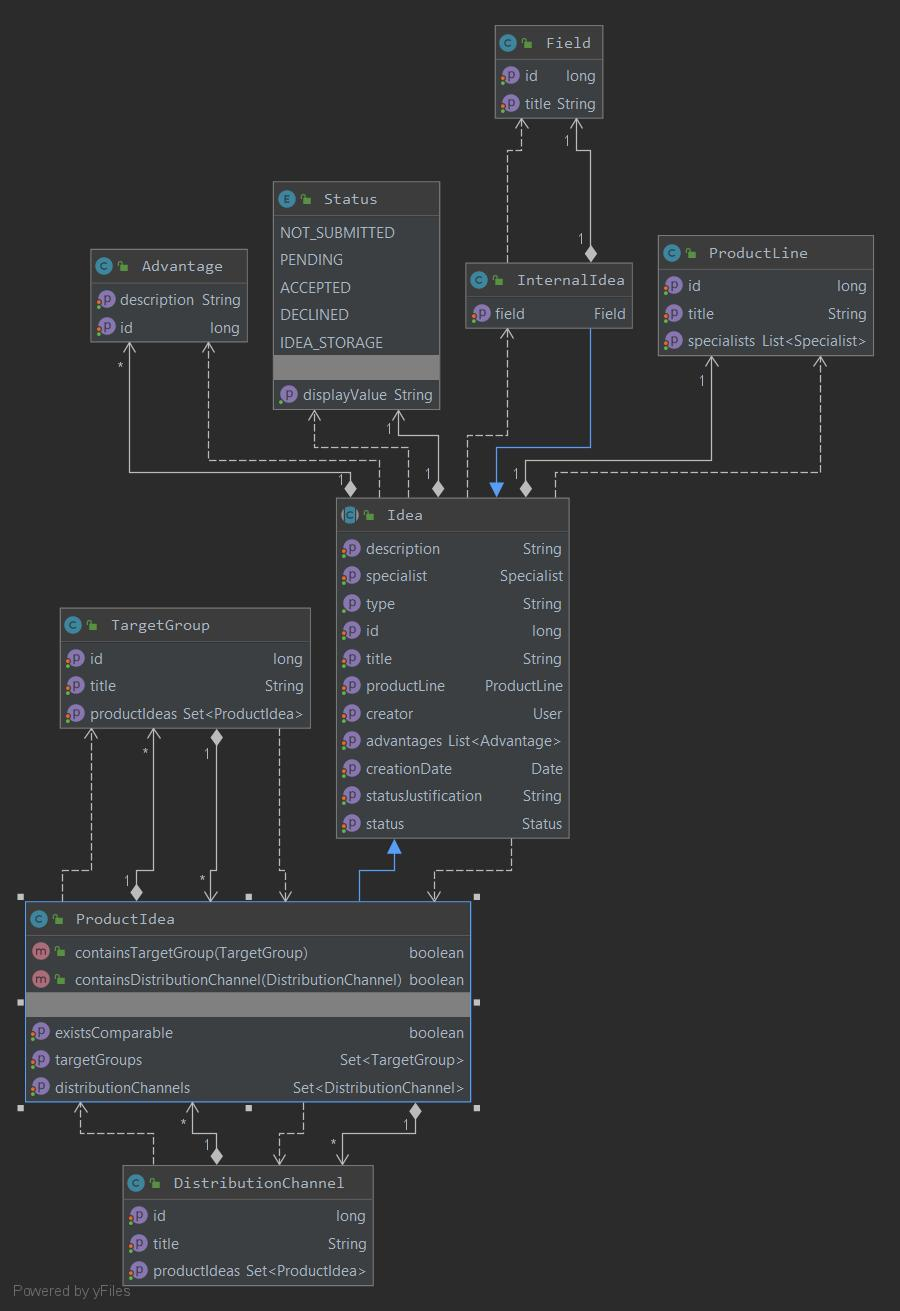
\includegraphics[width=0.7\textwidth]{img/idea-model-klassendiagramm.jpg}\\
        \source{Eigene Darstellung}
        \label{fig:idea-model-klassendiagramm}
    \end{minipage}
\end{figure}

\begin{figure}[htb]
    \centering
    \begin{minipage}[H]{1\textwidth}
        \caption{Klassendiagramm Model User}
        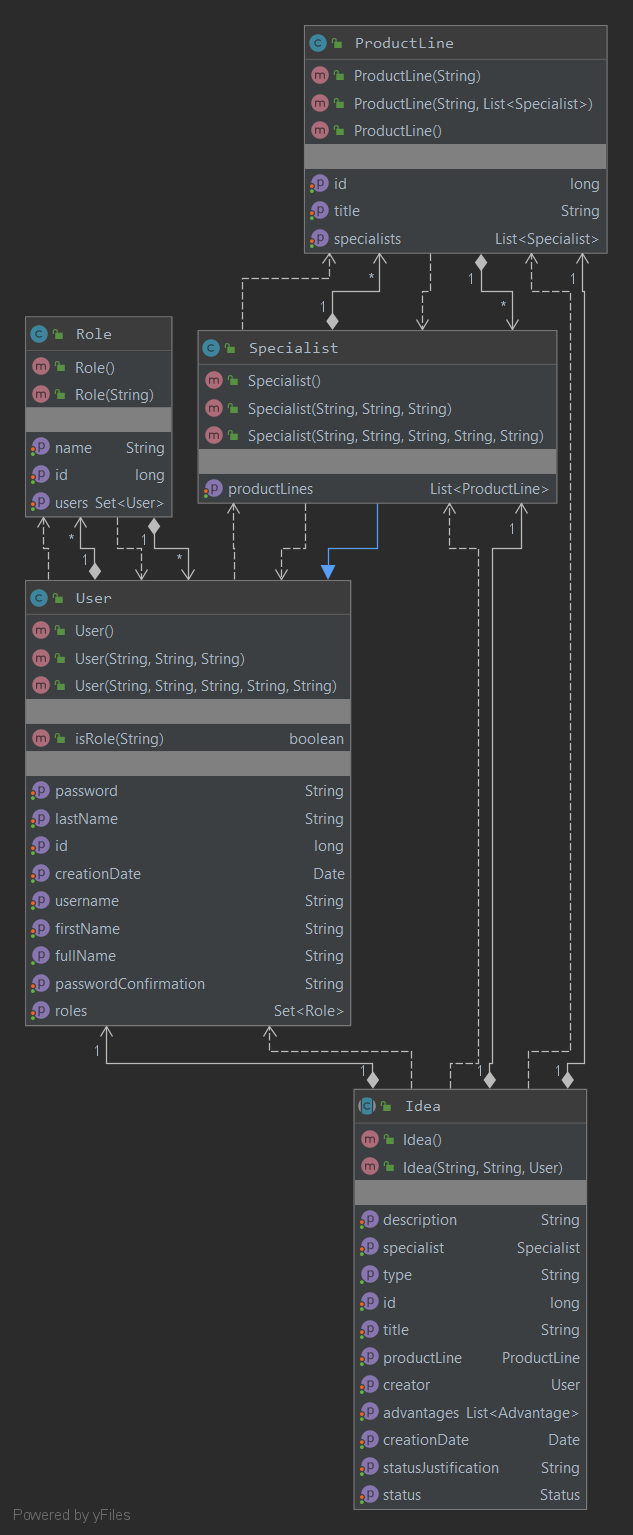
\includegraphics[width=0.55\textwidth]{img/user-model-klassendiagramm.png}\\
        \source{Eigene Darstellung}
        \label{fig:user-model-klassendiagramm}
    \end{minipage}
\end{figure}


%%%%%%%%%%%%%%%%%%%%%%%%%%%%%%%%%%%%%%%%%%%%%%%%%%%%%%%%%%%%%%%%%%%%%%%

    %!TEX root = ../Thesis.tex
\section*{Quellenverzeichnis}
\addcontentsline{toc}{section}{Quellenverzeichnis}
\fancyhead[R]{Quellenverzeichnis}

\defbibheading{mono}{\subsection*{Monographien}}
\defbibheading{mag}{\subsection*{Aufsätze in Sammelbänden und Zeitschriften}}
\defbibheading{art}{\subsection*{Zeitungsartikel}}
\defbibheading{web}{\subsection*{Internetquellen}}
\defbibheading{leg}{\subsection*{Rechtsprechung}}
\defbibheading{comp}{\subsection*{Unternehmensunterlagen/Gesprächsnotizen}}

\setlength\bibitemsep{1.5\itemsep}
\setlength{\bibhang}{2em}

\renewcommand{\baselinestretch}{1.50}\normalsize

\begingroup
\sloppy

\printbibliography[heading=web,keyword=web]

% Bei Bedarf einkommentieren: (erzeugt sonst Warnungen)
%\printbibliography[heading=mono,keyword=mono]
%\printbibliography[heading=mag,keyword=mag]
% \printbibliography[heading=art,keyword=art]
% \printbibliography[heading=leg,keyword=leg]
% \printbibliography[heading=comp,keyword=comp]

\endgroup

%%%%%%%%%%%%%%%%%%%%%%%%%%%%%%%%%%%%%%%%%%%%%%%%%%%%%%%%%%%%%%%%%%%%%%%


\end{document}
